\documentclass[11pt,a4paper]{article}

\usepackage[T1]{fontenc}
\usepackage[utf8]{inputenc}
\usepackage{lmodern}
\usepackage[margin=2.4cm]{geometry}
\usepackage{amsmath,amssymb}
\usepackage{booktabs}
\usepackage{tabularx}
\usepackage{longtable}
\usepackage{array}
\usepackage{xcolor}
\usepackage{listings}
\usepackage{microtype}
\usepackage{graphicx}
\usepackage[hidelinks]{hyperref}

\newcommand{\code}[1]{\texttt{#1}}
\setlength{\emergencystretch}{3em}
\newcommand{\up}{u_p}
\newcommand{\utau}{u_\tau}
\newcommand{\utp}{u_{\tau p}}
\newcommand{\dpds}{\partial p/\partial s}

\lstdefinelanguage{json}{
  morestring=[b]",
  literate={:}{{\textcolor{black}{:}}}1
}
\lstset{
  basicstyle=\ttfamily\footnotesize,
  columns=fullflexible,
  keepspaces=true,
  frame=single,
  rulecolor=\color{black!30},
  breaklines=true,
  stringstyle=\color{blue!50!black},
  showstringspaces=false
}

\title{Integration of the Reichardt and Duprat wall models\\into Neko (\code{feature/wmles})\\[0.5ex]
\large Work report}
\author{Prepared with Claude Code for M.~Münsch}
\date{12 October 2026, extended 27 October 2026}

\begin{document}
\maketitle

\begin{abstract}
This report documents the port of the Reichardt and the Duprat et al.\ wall
models from the \code{curved\_neko} fork (Master's thesis of D.~Bole) into
the \code{feature/wmles} branch of \code{muenschm/neko}, between 29 September
and 8 October 2026. The work was done in six pull requests, all merged.
Both models are now available on the CPU backend and, partially untested, on
the CUDA, HIP, OpenCL and Metal backends. The review of the original
implementation against the paper of Duprat et al.\ (2011) found several
issues, most importantly a spurious Jacobian factor in the pressure gradient
(``FIX~10'') that reduced the gradient seen by the model by a factor of
roughly 250--2700 on the periodic-hill mesh, and an inaccurate quadrature of
the velocity profile. The report records the findings, the decisions taken,
the implementation, the tests with their exact settings, and the open
items. The extension of 27 October covers a mesh-connectivity bug that
stopped Intel builds on more than one rank (fixed in PR~\#7), and the first
periodic-hill results at $Re_h = 10\,595$ with the Reichardt model on CPU
(Fritz) and GPU (Alex), compared with the LES database of Gloerfelt \&
Cinnella (2019). The recirculation zone comes out much too short: the flow
separates late and reattaches at $x/h \approx 2.7$--2.8 instead of
4.2--4.5. GPU and CPU agree in the mean flow, but the shear-layer
turbulence is 5--13\,\% higher on the GPU, which a deterministic test should
clarify.
\end{abstract}

\tableofcontents
\newpage

%=====================================================================
\section{Summary}
%=====================================================================

\begin{itemize}
  \item \textbf{Reichardt} (\code{"model": "reichardt"}): CPU (PR~\#1),
    CUDA/HIP/OpenCL/Metal (PR~\#2), configurable constants \code{C},
    \code{B1}, \code{B2} (PR~\#3).
  \item \textbf{Duprat} (\code{"model": "duprat"}): CPU with a constant
    prescribed pressure gradient (PR~\#4), locally evaluated and filtered
    pressure gradient (PR~\#5), CUDA/HIP/OpenCL/Metal for both modes
    (PR~\#6).
  \item The Duprat port follows the paper \cite{duprat2011} rather than the
    original code. Five issues of the original implementation were
    corrected (Section~\ref{sec:duprat-review}); two of them, the Jacobian
    factor and the quadrature, may affect the results reported in the
    thesis \cite{bole2026}.
  \item \textbf{GPU code:} the device code of both models was checked as
    follows.
    \begin{itemize}
      \item The device code was first verified on the host and, for OpenCL,
        by running Neko's full solver through PoCL.
      \item Since then, both models have run the full periodic hill on one
        NVIDIA GPU (Alex, CUDA).
      \item HIP and Metal have not run on hardware.
      \item The rank-0 warning that the GPU implementation is partially
        untested has been removed from both models on the upstream branches.
    \end{itemize}
  \item No spurious wall-normal velocity was found, on flat or curved walls
    (Section~\ref{sec:penetration}).
  \item A mesh-connectivity bug made Intel builds fail on more than one rank
    (\code{Invalid face neigh.}); it was fixed in PR~\#7 and is merged
    upstream as ExtremeFLOW/neko\#2867 (Section~\ref{sec:pr7}).
  \item \textbf{Periodic hill, Reichardt} (Section~\ref{sec:hill}).
    \begin{itemize}
      \item \emph{Mean flow:} the outer flow and the recovery region agree
        well with Gloerfelt \& Cinnella~\cite{gloerfelt2019}.
      \item \emph{Bubble:} the flow separates late ($x/h \approx 0.55$) and
        reattaches early ($x/h \approx 2.7$--2.8, reference 4.2--4.5).
        This is consistent with an equilibrium wall model that ignores the
        adverse pressure gradient at the crest, together with a coarse
        wall-normal resolution there.
      \item \emph{GPU versus CPU:} the runs agree in the mean flow, the skin
        friction and the separation point. The shear-layer turbulence was
        higher on the GPU. The Duprat runs, made with the same builds, do not
        show this, so it is probably not a code-path difference. A
        deterministic restart test is prepared to settle it.
    \end{itemize}
  \item \textbf{Periodic hill, Duprat} (Section~\ref{sec:hilldup}).
    \begin{itemize}
      \item \emph{Improvements over Reichardt:} the windward skin-friction
        peak now matches the reference (0.031 against 0.033). The flow
        separates earlier (0.45) and reattaches later (3.2--3.4).
      \item \emph{Remaining deficits:} the reattachment is still about 1
        short of the reference. Drag and skin friction are 33--43\,\%
        higher than with Reichardt.
      \item \emph{Cause:} in the bubble and in the recovery region the local
        mode passes on only about a tenth of the mean pressure gradient.
        Three improvements of the local mode are proposed.
      \item \emph{GPU versus CPU:} no systematic difference.
    \end{itemize}
  \item \textbf{Upstream:} both models are prepared as separate pull
    requests against ExtremeFLOW/neko \code{develop}, each with a pFUnit
    suite (Section~\ref{sec:open}).
\end{itemize}

\noindent Open items are listed in Section~\ref{sec:open}.

%=====================================================================
\section{Starting point}
%=====================================================================

\subsection{Repositories}

\begin{description}
  \item[\code{muenschm/neko}, branch \code{feature/wmles}] in sync with Neko
    \code{develop}; head at the start: \code{3837897} (``Update joblimit
    check \ldots\ (\#2817)'').
  \item[\code{muenschm/curved\_neko}, branch \code{feature/bc}] the
    student's work as a single commit \code{f2b81c1} (``Initial commit'',
    D.~Bole, 26 May 2026) on top of an older Neko \code{develop}
    (\code{a4aaf2c}). The commit contains 16 files (+3316/$-$10 lines):
    \begin{itemize}
      \item the models: \code{reichardt.f90}, \code{reichardt\_cpu.f90},
        \code{duprat.f90}, \code{duprat\_cpu.f90}, plus changes to
        \code{wall\_model\_fctry.f90} and \code{Makefile.am};
      \item build artefacts (\code{build\_curved/}: \code{libneko.lai},
        generated \code{neko.h}, \code{intf.py});
      \item a periodic-hill example including the 1.6\,MB mesh twice
        (\code{examples/periodic hill/} and its \code{run1/} copy).
    \end{itemize}
\end{description}

\subsection{API drift and porting strategy}

The wall-model API of Neko changed considerably between the student's base
and \code{feature/wmles}, mainly through upstream PR~\#2646 (``Wall model
sampling enhancements'', T.~Mukha, 20 August 2026):

\begin{center}
\small
\begin{tabularx}{\textwidth}{>{\raggedright}X>{\raggedright\arraybackslash}X}
\toprule
Student's base & \code{feature/wmles} \\
\midrule
\code{init(\ldots, h\_index, json)} &
  \code{init(\ldots, json)}; sampler from \code{wall\_sampler\_factory} \\
\code{ind\_r/s/t/e}, \code{h} in \code{wall\_model\_t} &
  \code{class(wall\_sampler\_t) :: sampler}, \code{sampler\%h} \\
\code{partial\_init(coef, json)} & \code{partial\_init(coef, scheme\_name, json)} \\
\code{finalize(msk, facet)} &
  \code{finalize(msk, facet, bc\_name, user)} + \code{validate\_single\_sample()} \\
CPU kernels index full $l_x^3 n_{el}$ fields &
  kernels work on pre-sampled vectors (\code{sampler\%sample}) \\
\bottomrule
\end{tabularx}
\end{center}

\noindent A merge or cherry-pick was therefore not possible. The models
were ported by hand, step by step, one pull request per testable step,
with \code{spalding} and \code{cai\_sagaut\_model\_ii} as templates.

%=====================================================================
\section{Workflow and pull requests}
%=====================================================================

All work was done on the branch \code{claude/stoic-euler-8zyrhx} of
\code{muenschm/neko}. After each merge, the branch was reset to the new
\code{feature/wmles}, so each PR contains exactly one step. The first push
failed (HTTP~403) until GitHub was reconnected for the session. All PRs were
reviewed and merged by M.~Münsch.

\begin{center}
\small
\begin{tabularx}{\textwidth}{@{}l>{\raggedright}Xllc@{}}
\toprule
PR & Title & Head & Merge commit & Merged \\
\midrule
\#1 & Add the Reichardt wall model (CPU backend) & \code{b0b064e} & \code{e95465a} & 30 Sep \\
\#2 & Add device backends for the Reichardt wall model & \code{382d1a9} & \code{29ff2d1} & 7 Oct \\
\#3 & Make the Reichardt constants configurable & \code{a23da72} & \code{d7978b5} & 8 Oct \\
\#4 & Add the Duprat wall model with a constant pressure gradient (CPU) & \code{62b734a} & \code{f419a96} & 8 Oct \\
\#5 & Duprat wall model: local pressure-gradient mode & \code{25155a4} & \code{ff1e65d} & 8 Oct \\
\#6 & Add device backends for the Duprat wall model & \code{1b5fbc0} & \code{b70f8d7} & 8 Oct \\
\bottomrule
\end{tabularx}
\end{center}

\noindent In total, 31 files changed (+5254/$-$3 lines) between
\code{3837897} and \code{b70f8d7}; see Appendix~\ref{app:files}.

%=====================================================================
\section{Reichardt wall model}
%=====================================================================

\subsection{Formulation}

Reichardt's law of the wall \cite{reichardt1951},
\begin{equation}
  u^+ = \frac{1}{\kappa}\ln(1+\kappa y^+)
      + C\left[1 - e^{-y^+/B_1} - \frac{y^+}{B_1}\,e^{-y^+/B_2}\right],
  \qquad C = 7.8,\; B_1 = 11,\; B_2 = 3,
  \label{eq:reichardt}
\end{equation}
is solved for $\utau$ from $f(\utau) = \utau\,u^+(h\utau/\nu) - U = 0$ with
Newton's method and the analytical derivative
$f' = u^+ + y^+\,\mathrm{d}u^+/\mathrm{d}y^+$. Here $U$ is the magnitude
of the sampled wall-parallel velocity. The wall stress is
$\boldsymbol\tau_w = -\rho_w\utau^2\,\mathbf{u}_t/|\mathbf{u}_t|$.

\subsection{CPU port (PR \#1)}

The port follows \code{spalding}. Differences to the original code:
\begin{itemize}
  \item The wall stress is scaled by the wall density $\rho_w$, consistent
    with the other wall models. This changes nothing for $\rho=1$.
  \item The parameter \code{B} was accepted but never used, so it was
    removed.
  \item OpenMP in the kernel, a zero-velocity guard, and a precision-aware
    Newton tolerance $\max(10^{-8}, 10\,\varepsilon_{\mathrm{mach}})$; with
    $10^{-8}$ alone, single precision would not converge.
\end{itemize}

\subsection{GPU kernels (PR \#2)}

CUDA and HIP (templated on the precision), OpenCL and Metal (FP32)
kernels, structured like \code{spalding} and \code{cai\_sagaut\_model\_ii}.
At M.~Münsch's request, the device backends print a rank-0 warning (``The
reichardt wall model GPU implementation is partially untested so far'')
instead of stopping with an error. After the hill runs on Alex
(Sections~\ref{sec:gpucpu} and~\ref{sec:hilldup-gpucpu}), this warning was
removed again on the upstream branches of both models.

\subsection{Configurable constants (PR \#3)}

To treat model constants consistently across wall models
(Section~\ref{sec:conventions}), $C$, $B_1$, $B_2$ became optional
case-file parameters \code{C}, \code{B1}, \code{B2}, with the defaults of
\eqref{eq:reichardt}. The names \code{B1}/\code{B2} were chosen by
M.~Münsch, to avoid confusion with coordinate directions (instead of the
proposed \code{y1}/\code{y2}).

\subsection{Verification}

\begin{itemize}
  \item \textbf{Kernels, known answer.} Sampled velocities constructed from
    a known $\utau$ for $y^+ = 0.5$--$500$ and $\rho_w\in\{1, 1.2\}$; the
    kernels recover $\utau$ to $8.7\times10^{-16}$ (double) and
    $7.5\times10^{-8}$ (single; $2.4\times10^{-7}$ for OpenCL). This was
    tested for:
    \begin{itemize}
      \item the CPU kernel;
      \item CUDA and HIP, compiled as host C++ with stubbed keywords;
      \item Metal, stubbed;
      \item OpenCL, the generated source JIT-compiled through PoCL.
    \end{itemize}
    The wall-normal velocity is removed, and zero velocity gives zero
    stress. After PR~\#3 the same tests also passed with a non-default set
    $(C, B_1, B_2) = (6, 9, 2.5)$.
  \item \textbf{Full solver.} \code{turb\_channel} example, $N=3$, 20 steps,
    $\Delta t = 0.01$; wall-model BC on zones 3 and 4, GLL sampling at
    index~2; force on the bottom wall:
    \begin{center}
    \small
    \begin{tabular}{lc}
      \toprule
      Case & $F_x$ \\
      \midrule
      \code{spalding} & $0.42830\times10^{-2}$ \\
      \code{reichardt} (CPU, unchanged after \#2) & $0.42879\times10^{-2}$ \\
      \code{reichardt}, explicit default constants (\#3) & $0.42879\times10^{-2}$ \\
      \code{reichardt}, $(C,B_1,B_2) = (6, 9, 2.5)$ & $0.44443\times10^{-2}$ \\
      \bottomrule
    \end{tabular}
    \end{center}
  \item \code{lint.sh} 10/10; \code{validate\_case\_schema.py} accepts valid
    cases and rejects a case without \code{kappa}.
\end{itemize}

%=====================================================================
\section{Duprat wall model}
%=====================================================================

\subsection{Formulation}
\label{sec:duprat-formulation}

Duprat et al.\ \cite{duprat2011} integrate the simplified thin-boundary-layer
equation across the wall layer, using an extended velocity scale. With
$\dpds$ the wall-tangential pressure gradient along the local flow
direction:
\begin{align}
  \up &= \left|\frac{\nu}{\rho}\frac{\partial p}{\partial s}\right|^{1/3},
  \qquad
  \utp = \sqrt{\utau^2 + \up^2},
  \qquad
  \alpha = \frac{\utau^2}{\utp^2},
  \qquad
  y^* = \frac{y\,\utp}{\nu},
  \label{eq:duprat-scales}\\
  \frac{\mathrm{d}U^*}{\mathrm{d}y^*} &=
    \frac{s_p\,(1-\alpha)^{3/2}\,y^* + \alpha}{1 + \nu_t/\nu},
  \label{eq:duprat-ode}\\
  \frac{\nu_t}{\nu} &= \kappa\,y^*\left[\alpha + y^*(1-\alpha)^{3/2}\right]^\beta
    \left(1 - e^{-y^*/(1+A\alpha^3)}\right)^2,
  \qquad \beta = 0.78,\; A = 17.
  \label{eq:duprat-nut}
\end{align}
Here $s_p$ is the sign of the pressure gradient relative to the flow
(adverse positive). Equations (4), (5) and (6) of the paper correspond to
\eqref{eq:duprat-scales}, \eqref{eq:duprat-ode} and \eqref{eq:duprat-nut}.
The paper writes the pressure velocity as
$\up = |(\mu/\rho^2)\,\partial P/\partial x|^{1/3}$, which is identical,
since Neko's \code{p} is the dynamic pressure: the pressure equation uses
$h_1 = 1/\rho$. The friction velocity follows from
$f(\utau) = \utp\,U^*(h\utp/\nu) - U = 0$. For $\dpds = 0$, $\alpha = 1$
and the model reduces to its equilibrium form.

\subsection{Review of the original implementation}
\label{sec:duprat-review}

The original code (\code{curved\_neko}) was compared with the paper, with the
thesis report \cite{bole2026}, and with Neko's operators.

\begin{center}
\small
\begin{longtable}{@{}p{0.2\textwidth}p{0.36\textwidth}p{0.36\textwidth}@{}}
\toprule
Item & Original code & Ported version \\
\midrule
\endhead
Pressure gradient (``FIX~10'') &
  \code{dudxyz}$(p)\times$\code{coef\%jac}, assuming \code{dudxyz} returns
  $(1/J)\,\partial p/\partial x$ &
  \code{grad}$(p)$, the physical gradient
  (Section~\ref{sec:fix10}) \\
$\up$ & $(\nu|\mathrm{d}p/\mathrm{d}x|/2)^{1/3}$ &
  $(\nu|\dpds|/\rho_w)^{1/3}$, Eq.~\eqref{eq:duprat-scales};
  also the form given in the report \\
Eddy viscosity & $(\kappa + \beta(1-\alpha)^{3/2})\,y^*(1-e^{\ldots})^2$ &
  Eq.~\eqref{eq:duprat-nut}; the report's listing also shows this form \\
Wall-stress term in \eqref{eq:duprat-ode} & $+1$ & $+\alpha$ \\
$U^*$ quadrature & one 5-point Gauss rule on $[0, y^*]$ &
  composite $12\times5$ Gauss rule in $\ln(1+y^*)$
  (Section~\ref{sec:quadrature}) \\
Solver & Newton; can collapse to $\utau\approx0$ for favourable gradients &
  root bracketed by sign change, Newton with bisection fallback \\
Gradient time level & $\nabla p^{\,n-1}$ (double buffer) with $\mathbf{u}^n$ &
  $\nabla p^{\,n}$, the same time level as $\mathbf{u}^n$
  (Section~\ref{sec:local}) \\
Streamwise gradient & $|\nabla_t p|\cdot\operatorname{sign}(\nabla_t p\cdot\mathbf{u}_t)$ &
  projection $\nabla p\cdot\mathbf{u}_t/|\mathbf{u}_t|$ \\
Stokes clamp & $|\dpds| \le 2(u\nu/h)^{3/2}/\nu$ &
  $|\dpds| \le (\rho_w/\nu)(u\nu/h)^{3/2}$, consistent with $\up$ \\
Filter & $\epsilon = \min(\Delta t/T, 0.5)\cdot\text{ramp}$, pre-activation buffer &
  $\epsilon = 1 - e^{-\Delta t/T}$, filtered value starting from zero \\
\bottomrule
\end{longtable}
\end{center}

\noindent The eddy-viscosity and $+1/+\alpha$ differences, as well as the
factor in $\up$, vanish for $\alpha = 1$. They therefore do not affect the
zero-pressure-gradient channel runs of the thesis. The temporal filter,
ramp and clamp are not part of the paper, which evaluates $\tau_w$ locally
from the filtered LES velocity in the first cell. They are numerical
stabilisation added by the student, and are kept as documented, adjustable
safeguards.

\subsection{The Jacobian factor (``FIX 10'')}
\label{sec:fix10}

The original code multiplied the output of \code{dudxyz} by
\code{coef\%jac}. Its comment states that \code{dudxyz} returns
$(1/J)\,\partial p/\partial x$ and that $J$ ``varies by factors 2--5''.
Both assumptions are incorrect:
\begin{itemize}
  \item \code{coef\%drdx} etc.\ are cofactors, i.e.\ $J\,\partial r/\partial x$
    (\code{sem/coef.f90}, around line 1146). \code{dudxyz} multiplies by
    \code{jacinv}, so its result is the physical gradient. Neko's own
    \code{curl} uses it that way (\code{opr\_cpu.f90}, lines 150--165).
  \item $J$ is not a ratio of order one but the volume scaling of the map
    from the reference element $[-1,1]^3$, i.e.\ about $1/8$ of the element
    volume.
\end{itemize}

\paragraph{Test.} On the student's periodic-hill mesh (\code{box.nmsh},
6688 elements, his mesh deformation, $N=7$), $p = x + 2y - 3z$ was set and
\code{dudxyz} applied:

\begin{center}
\small
\begin{tabular}{lccc}
\toprule
& $\partial p/\partial x$ & $\partial p/\partial y$ & $\partial p/\partial z$ \\
\midrule
\code{dudxyz} & 1.0000 (everywhere) & 2.0000 & $-3.0000$ \\
\code{dudxyz}$\times$\code{jac} (FIX 10) & $3.7\times10^{-4}$ -- $4.1\times10^{-3}$ & $7.4\times10^{-4}$ -- $8.2\times10^{-3}$ & -- \\
\bottomrule
\end{tabular}
\end{center}

\paragraph{Consequence.} With FIX~10 the model sees a pressure gradient
that is 250--2700 times too small. Since $\up\propto|\dpds|^{1/3}$, $\up$
is 6--14 times too small and $\alpha$ stays close to 1, so the
pressure-gradient correction is nearly switched off. This agrees with three
observations:
\begin{itemize}
  \item the code comment of FIX~10, which reports a CFL blow-up at
    $t = 110.5$ after the pressure gradient was switched on at
    $t_{\mathrm{filter,start}} = 100$; FIX~10 ``fixed'' it;
  \item the thesis conclusion that Duprat showed no systematic advantage
    over Reichardt on the periodic hill (Sections 6.1--6.2 of
    \cite{bole2026});
  \item the thesis report itself (Section 3.1.3) states correctly that
    \code{dudxyz} gives the physical gradient, and does not mention FIX~10.
\end{itemize}

\paragraph{Caveat.} The final committed code contains FIX~10, but which code
version produced the production runs of the thesis could not be
established from the documents. This should be confirmed with the student.

\paragraph{Decision.} FIX~10 was dropped. The gradient is computed with
Neko's \code{grad} (three \code{dudxyz} calls, with a device variant).

\subsection{Quadrature of $U^*$}
\label{sec:quadrature}

$U^*(y^*)$ was compared against SciPy's adaptive quadrature. As a check of
the formulation itself, the reference gives $U^*(1000) = 22.379$ at
$\alpha=1$, consistent with Fig.~3 of \cite{duprat2011} ($\approx 22.5$).

\begin{center}
\small
\begin{tabularx}{\textwidth}{@{}>{\raggedright}Xc>{\raggedright\arraybackslash}X@{}}
\toprule
Quadrature & worst rel.\ error in $U^*$ & comment \\
\midrule
single 5-point Gauss rule on $[0,y^*]$ (original) & up to 60\,\% & 48--60\,\% at $y^* \ge 10^3$, $\alpha=1$ \\
composite $8\times5$ Gauss in $\ln(1+y^*)$ & $8.6\times10^{-7}$ & \\
composite $12\times5$ Gauss in $\ln(1+y^*)$ (ported) & $5.8\times10^{-9}$ & \\
\bottomrule
\end{tabularx}
\end{center}

\noindent Tested for $\alpha\in\{1, 0.7, 0.3, 0.05\}$, adverse and
favourable gradients, and $y^*$ up to $10^4$. At $\alpha = 1$ and the
sampling heights of the thesis channel runs, the original rule gives:

\begin{center}
\small
\begin{tabular}{ccc}
\toprule
$y^*$ & exact $U^*$ & original rule \\
\midrule
33.3 & 13.945 & 13.945 ($-0.0$\,\%) \\
60   & 15.568 & 15.421 ($-0.9$\,\%) \\
153  & 17.832 & 19.308 ($+8.3$\,\%) \\
\bottomrule
\end{tabular}
\end{center}

\noindent The thesis reports an 8.4\,\% DNS mismatch of Duprat at
\code{h\_index}~=~7 ($y^+\approx153$) and attributes it to the model's
velocity profile. The close agreement with the $+8.3$\,\% quadrature error
suggests that this deterioration is, at least partly, a quadrature
artefact.

\subsection{Constant pressure gradient on CPU (PR \#4)}

\begin{itemize}
  \item \code{kappa} is required; \code{beta} (0.78) and \code{A} (17) are
    optional.
  \item The pressure gradient is set by the optional object
    \code{"pressure\_gradient": \{"type": "constant", "value": \ldots\}};
    without it, the gradient is zero (equilibrium limit). \code{value} is
    $\dpds$ along the local flow direction, positive if adverse. It
    replaces the student's pair \code{use\_constant\_dpdx: true} /
    \code{dpdx\_constant} (Appendix~\ref{app:mapping}).
  \item The residual is not monotone in $\utau$ for favourable gradients:
    it first decreases, then increases. A root always exists ($f(0)<0$,
    $f\to\infty$), but plain Newton walks into the decreasing branch and
    gives $\utau\approx0$. The solver therefore first brackets the root by
    a sign change and replaces Newton steps that leave the bracket by
    bisection.
\end{itemize}

\paragraph{Verification.}
\begin{itemize}
  \item 96 known-answer cases (velocity from the SciPy integral for a known
    $\utau$): $y^+\in[1, 2000]$, $\up/\utau\in\{0, 0.3, 1, 2, 5\}$,
    adverse and favourable, $\rho\in\{1, 1.3\}$. Maximum relative error of
    $\utau$: $1.2\times10^{-7}$ (double) and $1.4\times10^{-5}$ (single).
    Cases where the model gives $U<0$ (strong favourable gradient) were
    excluded, since a velocity magnitude cannot be negative.
  \item 48 strong favourable-gradient cases: a true root is found in every
    case, $|f|/U < 7\times10^{-14}$, where the plain Newton solver gave
    $\utau\approx0$.
  \item \code{turb\_channel}, $N=3$, 20 steps, GLL sampling index 2, bottom
    wall force:
    \begin{center}
    \small
    \begin{tabular}{lc}
      \toprule
      Case & $F_x$ \\
      \midrule
      \code{reichardt} & $0.42879\times10^{-2}$ \\
      \code{duprat}, zero gradient & $0.42872\times10^{-2}$ \\
      \code{duprat}, $\dpds = -0.0036$ ($\approx -\utau^2/\delta$) & $0.43835\times10^{-2}$ ($+2.2$\,\%) \\
      \code{duprat}, \code{"type": "local"} (before PR \#5) & rejected with an error \\
      \bottomrule
    \end{tabular}
    \end{center}
    The favourable gradient flattens the near-wall profile, so the same
    sampled velocity implies a higher wall stress.
  \item The same runs with the legacy \code{"h\_index": 2} instead of
    \code{"sampling": \{"type": "gll", "value": 2\}} give identical forces
    (Section~\ref{sec:conventions}).
\end{itemize}

\subsection{Local pressure gradient (PR \#5)}
\label{sec:local}

\paragraph{Timing.} In \code{fluid\_pnpn\_step}, the wall stress is computed
once per time step, when the Neumann contributions are added to the
right-hand side (\code{fluid\_pnpn.f90}, line 758). This happens
\emph{before} the pressure and velocity solves. When $\tau_w$ for step
$n+1$ is computed, the newest fields are therefore $\mathbf{u}^n$ and
$p^n$. The original code used $\nabla p^{\,n-1}$ with $\mathbf{u}^n$. As
suggested by M.~Münsch, the ported version uses $\nabla p^{\,n}$, the same
time level as the sampled velocity. Using $p^{n+1}$ is not possible without
restructuring the solver.

\paragraph{Per time step.}
\begin{enumerate}
  \item $\nabla p$ with \code{grad} (physical gradient, no Jacobian factor);
  \item sampling of the three components through the model's
    \code{sampling}, at the same points as the velocity;
  \item projection on the local flow direction,
    $\dpds = \nabla p\cdot\mathbf{u}_t/|\mathbf{u}_t|$ (the paper's
    streamwise gradient; the magnitude of the full tangential gradient
    would also pick up spanwise fluctuations);
  \item Stokes limit $|\dpds| \le (\rho_w/\nu)(u\nu/h)^{3/2}$, i.e.\
    $\up \le \sqrt{u\nu/h}$;
  \item exponential moving average, as decided by M.~Münsch:
    \begin{equation}
      \left(\dpds\right)_{\mathrm{filt}}^{n} =
        (1-\epsilon)\left(\dpds\right)_{\mathrm{filt}}^{n-1}
        + \epsilon\left(\dpds\right)^{n},
      \qquad \epsilon = 1 - e^{-\Delta t/T}.
      \label{eq:ema}
    \end{equation}
    This weight is the exact discrete form of a first-order low-pass filter
    for variable $\Delta t$; $T = 0$ gives $\epsilon = 1$ (no filtering).
\end{enumerate}

\noindent The update is done once per time step. Before \code{start\_time}
the filtered gradient stays zero. Since it starts from zero, it enters over
about one filter time; the student's separate ramp and pre-activation
buffer are therefore not needed.

\paragraph{Case file.}
{\sloppy
\code{"pressure\_gradient":} \code{\{"type": "local",} \code{"filter\_time": $T$,}
\code{"start\_time": $t_0$\}}. \code{filter\_time} is
required, because it is dimensional and no default is meaningful;
\code{start\_time} defaults to 0.\par}

\paragraph{Diagnostics.} The filtered $\dpds$ and $\alpha$ at the wall
nodes are stored in the registry fields \code{duprat\_dpds} and
\code{duprat\_alpha}, like \code{tau}, and can be written with
\code{field\_writer}.

\paragraph{Limitation.} The filter state is not checkpointed. After a
restart it starts again from zero.

\paragraph{Verification.}
\begin{itemize}
  \item \textbf{Update kernel, exact checks:}
    \begin{itemize}
      \item projection, including removal of the wall-normal velocity and
        gradient components;
      \item sign for forward and reversed flow;
      \item clamp equal to the Stokes bound (31.62 in the test);
      \item a node without flow keeps its previous value;
      \item the filter reproduces $G(1-e^{-t/T})$ for constant input to
        $6\times10^{-14}$ over 200 steps.
    \end{itemize}
  \item \textbf{Known answer in a full run.} A user \code{preprocess} hook
    overwrote $p = G(x\cos\varphi + z\sin\varphi)$ before each step
    ($G = 0.05$, $\varphi = 60^\circ$), in uniform flow along $x$, so the
    expected $\dpds = 0.025$ at all 10\,368 wall nodes:
    \begin{itemize}
      \item without filter: 0.02500 from the second step on, maximum
        deviation $2.5\times10^{-6}$;
      \item $T = 0.05$, $t_0 = 0.035$: zero before $t_0$, then
        \eqref{eq:ema} step by step, maximum deviation
        $1.3\times10^{-6}$.
    \end{itemize}
  \item \textbf{Turbulent channel}, $N=3$, 200 steps, $T=1$:
    \begin{itemize}
      \item stable;
      \item $F_x = 0.37652\times10^{-2}$ vs $0.37222\times10^{-2}$ with zero
        gradient ($+1.2$\,\%);
      \item filtered $\dpds$ about $\pm0.03$--$0.04$, mean
        $-4\times10^{-4}$, as expected in a body-force-driven channel;
      \item $\alpha$ mostly $> 0.6$; one node reached $\alpha\approx0$
        transiently at step~60 (the model's local separation limit) and
        recovered.
    \end{itemize}
  \item The schema rejects \code{local} without \code{filter\_time}, and
    filter settings combined with \code{constant}.
\end{itemize}

\subsection{GPU kernels (PR \#6)}

Two kernels per backend, \code{duprat\_compute} and
\code{duprat\_update\_dpds}, mirroring the CPU kernels; plus device paths
in \code{duprat.f90}:
\begin{itemize}
  \item gathering $\nu$ and $\rho$ at the wall;
  \item \code{grad} on device pointers;
  \item vector fills;
  \item the masked scatter into the diagnostic fields.
\end{itemize}
The CPU-only error was replaced by the rank-0 ``partially untested''
warning.

\paragraph{Robustness fix (CPU and GPU).} $\alpha$ is formed as
$\utau^2/(\utau^2+\up^2)$ instead of $\utau^2/\utp^2$, and $1-\alpha$ is
limited to $\ge0$ before the power $3/2$. With relaxed GPU math, e.g.\
Metal fast math, rounding could otherwise give $\alpha$ slightly above 1
and NaN. On IEEE hardware the results are unchanged; no case with
$\alpha > 1$ occurred in $2\times10^5$ random samples in either precision.

\paragraph{Verification.}
\begin{center}
\small
\begin{tabular}{lccc}
\toprule
Kernel & known $\utau$: rel.\ error $\utau$ ($\alpha$) & favourable cases & update kernel \\
\midrule
CPU (reference) & $1.2\times10^{-7}$ ($8.8\times10^{-9}$) & root found & exact \\
CUDA/HIP, host C++, double & $1.2\times10^{-7}$ ($8.8\times10^{-9}$) & $|f|/U\le10^{-14}$ & $3\times10^{-16}$ \\
CUDA/HIP, host C++, float & $1.4\times10^{-5}$ ($1.0\times10^{-6}$) & $\le4\times10^{-6}$ & $8\times10^{-8}$ \\
Metal (stubbed), float & $1.4\times10^{-5}$ ($1.0\times10^{-6}$) & $\le4\times10^{-6}$ & $8\times10^{-8}$ \\
OpenCL via PoCL, double & $1.2\times10^{-7}$ ($8.8\times10^{-9}$) & finite, non-zero & $3\times10^{-16}$ \\
OpenCL via PoCL, float & $1.0\times10^{-5}$ ($7.4\times10^{-7}$) & finite, non-zero & $8\times10^{-8}$ \\
\bottomrule
\end{tabular}
\end{center}

\noindent \textbf{Full solver on the OpenCL backend.} PoCL does not
implement \code{clEnqueueWaitForEvents}. For this test only, a preloaded
shim replaced it by the blocking \code{clWaitForEvents}; Neko's sources
were not changed. The turbulent channel ($N=3$, 30 steps, one rank) gave:
\begin{center}
\small
\begin{tabular}{lccc}
\toprule
Case & $F_x$ CPU & $F_x$ OpenCL & $\dpds$, $\alpha$ at the wall \\
\midrule
zero gradient & $0.43246\times10^{-2}$ & $0.43246\times10^{-2}$ & identical \\
constant $\dpds = -0.0036$ & $0.44200\times10^{-2}$ & $0.44200\times10^{-2}$ & identical \\
\code{local}, $T = 0.05$ & $0.45788\times10^{-2}$ & $0.45788\times10^{-2}$ & identical \\
\bottomrule
\end{tabular}
\end{center}
In the \code{local} case, $\dpds\in[-0.187, 0.198]$ and
$\alpha\in[0.116, 1]$. Every reported value above $10^{-6}$ is identical at
every step; only the spanwise force ($\sim10^{-10}$) differs, by at most
$10^{-12}$.

%=====================================================================
\section{Case-file conventions}
\label{sec:conventions}
%=====================================================================

\paragraph{Model constants.} The existing models follow two conventions:

\begin{center}
\small
\begin{tabular}{lll}
\toprule
Model & \code{kappa} & further constants \\
\midrule
\code{spalding} & required & \code{B} required \\
\code{cai\_sagaut\_model\_ii} & required & \code{B} required; \code{p}, \code{s} optional (paper defaults) \\
\code{rough\_log\_law}, \code{most}, \code{richardson} & optional (0.4) & \code{B} optional (0) \\
\code{reichardt} (new) & required & \code{C}, \code{B1}, \code{B2} optional (7.8, 11, 3) \\
\code{duprat} (new) & required & \code{beta}, \code{A} optional (0.78, 17) \\
\bottomrule
\end{tabular}
\end{center}

\noindent The new smooth-wall models follow \code{cai\_sagaut\_model\_ii}:
log-law constants are required, model-specific calibration constants are
optional with paper defaults, and no constant is hardcoded. The
atmospheric-boundary-layer models were left unchanged, since changing them
would break existing case files.

\paragraph{Sampling.} \code{sampling} is the documented successor of
\code{h\_index} (upstream PR~\#2646: ``the now legacy \code{h\_index}
remains supported''). All wall models go through the shared
\code{wall\_sampler\_factory}, which uses \code{sampling} if present and
falls back to \code{h\_index} otherwise; this was confirmed by identical
results. The new documentation uses \code{sampling}, as decided by
M.~Münsch. \code{sampling} also allows \code{"type": "distance"}, and in the
\code{local} mode the pressure gradient goes through the same sampler as
the velocity.

%=====================================================================
\section{Wall-normal velocity (penetration) check}
\label{sec:penetration}
%=====================================================================

The wall-model boundary condition is a \code{shear\_stress} condition of
type\\ \code{BC\_MIXED\_CONSTRAINS\_NORMAL}. With a coupled velocity solver
(e.g.\ \code{coupled\_cg}), Neko's \code{vector\_bc\_projector} builds a
local basis $(\mathbf{n}, \mathbf{t}_1, \mathbf{t}_2)$ at each wall node and
constrains the normal component strongly. At element edges and corners it
uses an averaged node normal (face normals summed, gather-scatter,
normalised). The wall model only sets the tangential stress.

\begin{center}
\small
\begin{tabular}{lcc}
\toprule
Measure of $\mathbf{u}\cdot\mathbf{n}$ & Duprat \code{local}, $T=0$ & Reichardt \\
\midrule
Channel, all 10\,368 wall nodes, 100 steps & $\le1.3\times10^{-15}$ & -- \\
Hill, curved wall, facet-interior nodes & $\le4\times10^{-16}$ & $\le7\times10^{-16}$ \\
Hill, curved wall, averaged node normal, all nodes & $\le6\times10^{-16}$ & $\le7\times10^{-16}$ \\
Hill, curved wall, per-element normals, all nodes & $\approx0.02$ max, 0.003 RMS & same \\
Hill, net flux $\int\mathbf{u}\cdot\mathbf{n}\,\mathrm{d}A/A$ & $\sim3\times10^{-6}$ & $\sim5\times10^{-6}$ \\
\bottomrule
\end{tabular}
\end{center}

\noindent Settings for the hill: the student's mesh at $N=4$, uniform
initial flow along $x$ (which initially crosses the curved wall), GLL
sampling index 2. The per-element measure was run up to $t = 1$ (142 steps
for Duprat, 174 for Reichardt), the refined measures (facet-interior nodes,
averaged normal, net flux) up to $t = 0.3$ (40 steps). On the flat top wall
$|\mathbf{u}\cdot\mathbf{n}| \le 1.5\times10^{-14}$.

\paragraph{Interpretation.} The constraint is satisfied to round-off
everywhere. The $\approx1$\,\% residual with per-element normals is a
measurement artefact: on a curved wall, neighbouring elements meet with a
slight kink (continuous geometry, discontinuous slope), so their face
normals differ at shared edge nodes. The small net flux has the same origin,
since the surface integral uses face normals. It does not grow
systematically and should decrease at higher polynomial order. The behaviour
is the same for both models, so Duprat's pressure-gradient feedback plays
no part.

\paragraph{Related detail.} At edge nodes the wall models distribute
$\tau_w$ along the facet tangent of one element rather than the averaged
tangent. Any normal part is removed by the constraint (a 1\,\% effect, edge
nodes only). Using the projector's averaged normals would be cleaner, but
this belongs to Neko's wall-model base class.

%=====================================================================
\section{Multi-rank failure on Fritz: \code{Invalid face neigh.} (PR \#7)}
\label{sec:pr7}
%=====================================================================

\paragraph{Symptom.} The periodic hill ran on a desktop (gfortran, OpenMPI~5,
14 ranks). On Fritz (NHR@FAU; Intel compiler, OpenMPI~5 with UCX) every run on
more than one rank stopped during the mesh connectivity setup with
\code{*** ERROR: Invalid face neigh. ***}. The plain \code{mesh\_checker}
failed in the same way on 14 and 72 ranks, so neither the case file nor the
wall model was involved. A serial run worked, and the mesh was identical on
both machines (same element, point, face and edge counts).

\paragraph{Cause.} \code{mesh\_generate\_external\_facet\_conn} and
\code{mesh\_generate\_facet\_numbering} in \code{src/mesh/mesh.f90} passed
the result of the stack's \code{\%array()} function directly as the buffer of
the nonblocking \code{MPI\_Issend}. A compiler may pass a function result
through a temporary copy that is freed right after the call, while the
synchronous send is still pending. The receiving rank then gets corrupted
facet data, e.g.\ a neighbour element~0, and the consistency check of the
facet numbering stops the run. \code{mesh\_generate\_edge\_conn} in the same
file already avoids this pattern, with the comment that it ``breaks horribly
on Cray''.

\paragraph{Fix.} Both sends now pass the stack's own storage through
\code{select type}, as the edge exchange does. No other nonblocking MPI call
in \code{src} passes a function result as its buffer. With the fix,
\code{mesh\_checker} on 72 ranks completed on Fritz. In the container
(gfortran, OpenMPI~4.1.6), \code{mesh\_checker} completed on 2 to 144 ranks
for three periodic box meshes, and the forces of the periodic hill with and
without the fix differ only at the level of run-to-run variation. Merged into
\code{feature/wmles} as PR~\#7. The bug was also present on upstream
\code{develop}; the same change, prepared on the branch
\code{fix/mesh-issend-buffer}, is merged there as ExtremeFLOW/neko\#2867.

%=====================================================================
\section{Periodic hill at $Re_h = 10\,595$ with the Reichardt model}
\label{sec:hill}
%=====================================================================

\subsection{Case and runs}

\begin{itemize}
  \item \textbf{Geometry and mesh:} hill geometry of Breuer et al.\ as in the
    ERCOFTAC case, $L_x = 9h$, $L_y = 3.035h$, $L_z = 4.5h$. The
    \code{genmeshbox} mesh has $22\times8\times19$ elements, periodic in $x$
    and $z$; the user file maps it to the hill. With $N = 8$ this gives
    1.74~million unique points, about $176\times64\times152$. There is only
    weak stretching towards the walls: 8 elements over the channel height.
  \item \textbf{Flow:} $Re_h = 10\,595$. \code{flow\_rate\_force} sets the
    bulk velocity at the hill crest to $U_b = 1$; the value
    $0.720958 = 2.035/H_\mathrm{mean}$ was checked against the mean channel
    height. This is the definition used by Gloerfelt \&
    Cinnella~\cite{gloerfelt2019}; the evaluation confirms
    $U_b = 0.9999$.
  \item \textbf{Models and numerics:} Vreman ($c = 0.07$), gradient jump
    penalty (0.8, as a source term), \code{coupled\_cg} for the velocity,
    variable $\Delta t$ at CFL~0.5.
  \item \textbf{Wall model:} Reichardt on both walls ($\kappa = 0.41$,
    $C = 7.8$, $B_1 = 11$, $B_2 = 3$), sampling at GLL index~3. On the hill
    wall this gives $h_s = 0.062\ldots0.109\,h$.
  \item \textbf{Fixes to the student's case:} two settings in it were
    silently ignored by the current Neko:
    \begin{itemize}
      \item the old \code{gradient\_jump\_penalty} block, so the runs would
        have had no GJP;
      \item the Vreman keys \code{c\_s} and \code{field\_name}.
    \end{itemize}
    Both were corrected (\code{periodic\_hill/CHANGES.md}).
  \item \textbf{Output:}
    \begin{itemize}
      \item \code{force\_torque} on both walls every 10 steps, scaled with
        $2/(\rho U_b^2 L_x L_z)$. The scaled pressure and viscous parts are
        then the drag and skin-friction coefficients.
      \item \code{fluid\_stats} averaged over $z$
        (\code{"avg\_direction": "z"}), sampled every 10 steps from $t = 150$
        and written every 50 time units.
    \end{itemize}
\end{itemize}

\noindent Two runs with the same case file reached $t = 600$:

\begin{center}
\small
\begin{tabularx}{\textwidth}{@{}lX@{}}
\toprule
Run & Set-up \\
\midrule
Fritz (CPU) & Intel build with PR~\#7, OpenMPI~5, 72 ranks (one node).
Restarted at $t = 173.6$. After a restart Neko's statistics start again at
the restart time, so the statistics cover $t = 173.6\ldots600$, 47 flow-through
times $L_x/U_b$. \\
Alex (GPU) & GNU build, CUDA, one GPU. Restarted at $t = 100$; statistics
$t = 150\ldots600$, 50 flow-through times. \\
\bottomrule
\end{tabularx}
\end{center}

\noindent For comparison, Gloerfelt \& Cinnella averaged over 55--80
flow-through times after 23 for the transient.

\subsection{Evaluation}

Two scripts in \code{periodic\_hill/analysis} do the evaluation.
\code{ph\_stats.py} reads the 2D statistics files and combines the output
windows weighted with their lengths. The Reynolds stresses are formed from the
combined raw moments. The script interpolates the profiles spectrally inside
the elements at $x/h = 0.05, 0.5, 1, \ldots, 8$; the interpolation was checked
to round-off on the coordinates. \code{ph\_forces.py} evaluates the forces,
the forcing and the time stepping from the logs. Uncertainties are the
standard errors of the means over windows of 50 time units. These windows
are not fully independent, so the uncertainties are lower bounds.

The skin friction is not part of the statistics. The script reconstructs it
the way the wall model computes $\tau_w$: the mean velocity tangential to the
wall is taken at the sampling point, and Reichardt's law is solved for
$u_\tau$. This gives $\tau_w(\langle u\rangle)$, not
$\langle\tau_w\rangle$. Its magnitude is therefore approximate: the mean
$C_f$ obtained this way is 8\,\% (top wall) to 17\,\% (hill wall) below
the \code{force\_torque} value (Table~\ref{tab:hillforces}). Its sign, and with it the separation and
reattachment points, follows the mean flow.

The reference is the LES database of Gloerfelt \&
Cinnella~\cite{gloerfelt2019} at $Re_h = 10\,595$: $C_f$ on four grids from
$64\times33\times32$ to $512\times256\times256$, and profiles. The
experimental reattachment point of Rapp \& Manhart~\cite{rapp2011} is
$x/h = 4.21$.

\subsection{Forces and momentum balance}

\begin{table}[htbp]
\centering
\small
\caption{Time-averaged forces, scaled with $2/(\rho U_b^2 L_x L_z)$, and the
flow-rate forcing $f$. Full averaging range of each run; $\pm$ standard error
over windows of 50 time units.}
\label{tab:hillforces}
\begin{tabular}{@{}lcc@{}}
\toprule
 & Fritz (CPU), $t\ge173.6$ & Alex (GPU), $t\ge150$ \\
\midrule
hill wall, pressure drag $F_{x,p}$ & $0.0434 \pm 0.0009$ & $0.0449 \pm 0.0005$ \\
hill wall, skin friction $F_{x,v}$ & $0.00202 \pm 0.00006$ & $0.00212 \pm 0.00003$ \\
top wall, skin friction $F_{x,v}$ & $0.00616 \pm 0.00006$ & $0.00605 \pm 0.00004$ \\
reconstructed mean $C_f$, hill / top wall & 0.00169 / 0.00566 & 0.00176 / 0.00555 \\
forcing $\langle f\rangle$ & 0.00906 & 0.00932 \\
balance $\langle F_{x,3} + F_{x,4}\rangle / (2H_\mathrm{mean}\langle f\rangle)$ & 1.009 & 1.008 \\
\bottomrule
\end{tabular}
\end{table}

The pressure drag dominates the force on the hill wall; its skin friction is
only about 5\,\% of the total. The momentum balance closes to within 1\,\% in
both runs. The remainder reflects that \code{force\_torque} evaluates the
resolved wall gradient, while the wall model imposes the traction only
weakly. For comparison, the mean $C_f$ of the hill wall in the reference is
0.00132 on the finest grid and 0.0007--0.0011 on the coarser ones.
Figure~\ref{fig:hillforces} shows the time series.

\begin{figure}[htbp]
\centering
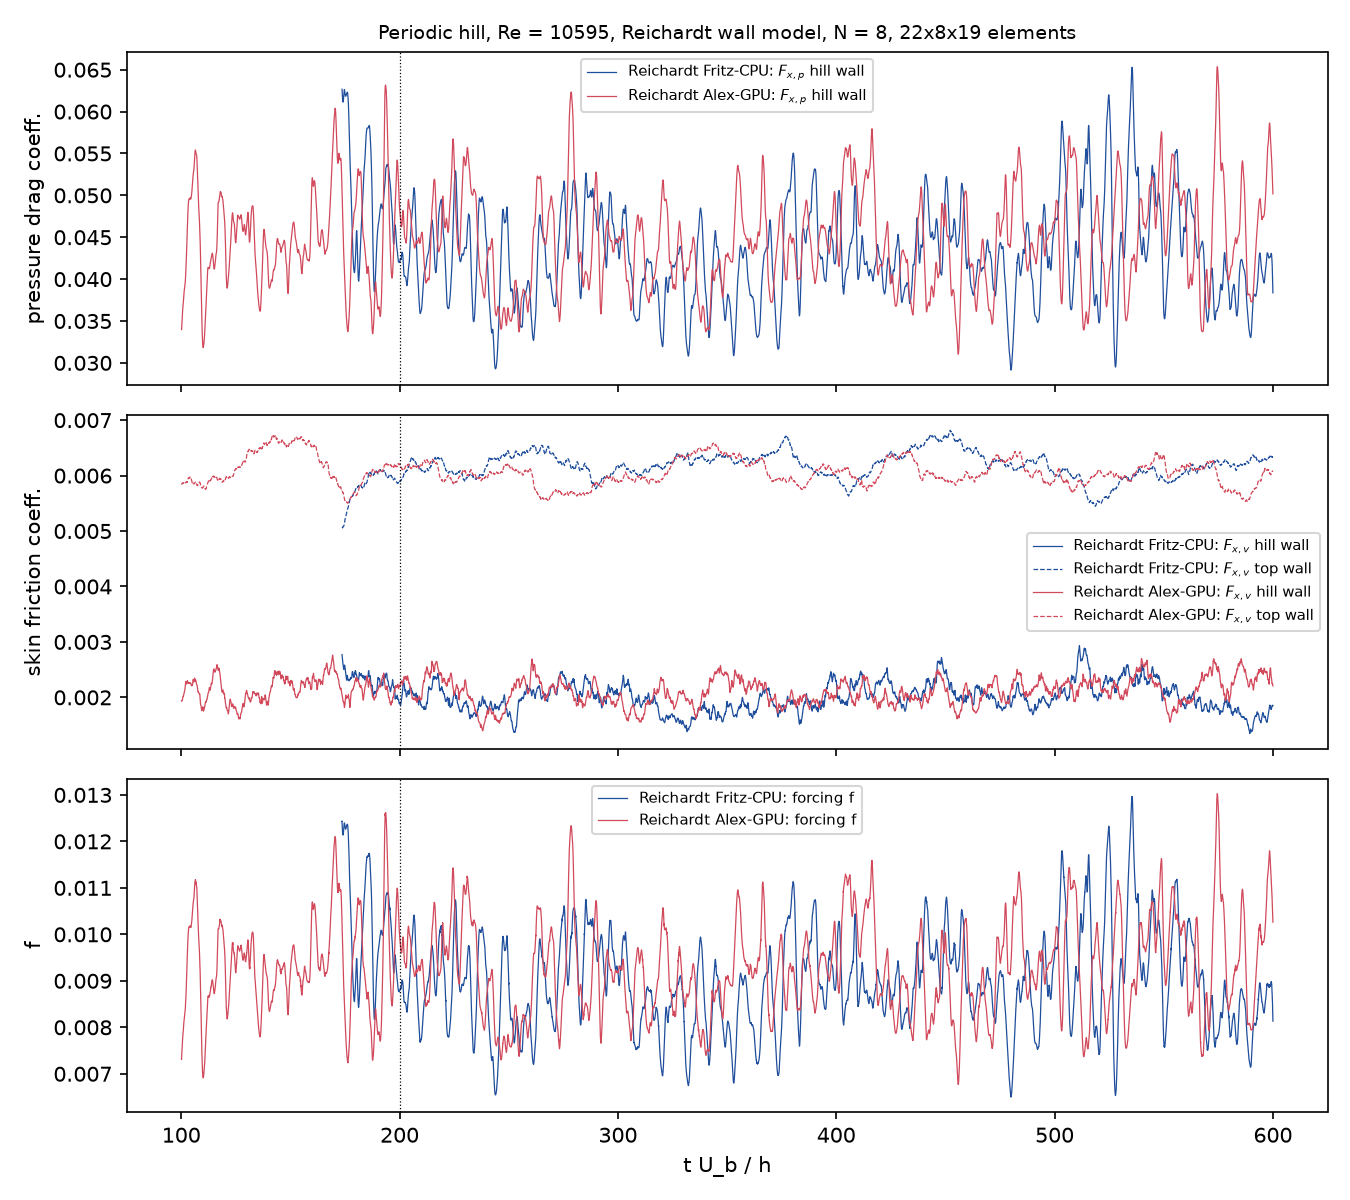
\includegraphics[width=0.85\textwidth]{figures/forces_time_Reichardt.png}
\caption{Forces and forcing over time, Reichardt model, Fritz (CPU) and Alex
(GPU). The dotted line marks $t = 200$, the start of the common averaging
range used in Section~\ref{sec:gpucpu}.}
\label{fig:hillforces}
\end{figure}

\subsection{Skin friction, separation and reattachment}

\begin{table}[htbp]
\centering
\small
\caption{Zero crossings of $C_f$ on the hill wall. Neko: reconstructed $C_f$,
full averaging range. The reference values are from the $C_f$ data of the
database.}
\label{tab:hillsep}
\begin{tabular}{@{}lcccc@{}}
\toprule
 & separation & reattachment & secondary bubble & $C_{f,\max}$ (windward) \\
\midrule
Neko Reichardt, Fritz (CPU) & 0.55 & 2.78 & -- & 0.011 \\
Neko Reichardt, Alex (GPU) & 0.55 & 2.71 & -- & 0.012 \\
Gloerfelt $512\times256\times256$ & $-0.12$ & 4.31 & 6.74--7.08 & 0.033 \\
Gloerfelt $256\times128\times128$ & $-0.16$ & 4.32 & 6.78--7.02 & 0.030 \\
Gloerfelt $128\times64\times64$ & $-0.11$ & 4.49 & -- & 0.023 \\
Gloerfelt $64\times33\times32$ & 0.24 & 4.31 & -- & 0.015 \\
Experiment (Rapp \& Manhart) & & 4.21 & & \\
\bottomrule
\end{tabular}
\end{table}

The recirculation zone is much too short (Table~\ref{tab:hillsep},
Figure~\ref{fig:hillcf}). The flow stays attached over the crest with
$C_f \approx 0.009\ldots0.010$, separates only at $x/h \approx 0.55$ and reattaches
already at $x/h \approx 2.7$--2.8, against 4.3--4.5 in all reference grids.
Over the reattachment points of the individual windows the scatter is about
$\pm 0.2$ (Fritz) and $\pm 0.1$ (Alex), so the difference is not
statistical. Inside the bubble, $C_f$ only reaches about $-0.0007$ against
$-0.002\ldots-0.004$. The peak on the windward face, 0.011--0.012, is close
to that of the coarsest reference grid, but the reconstruction from the mean
velocity underestimates peaks.

\begin{figure}[htbp]
\centering
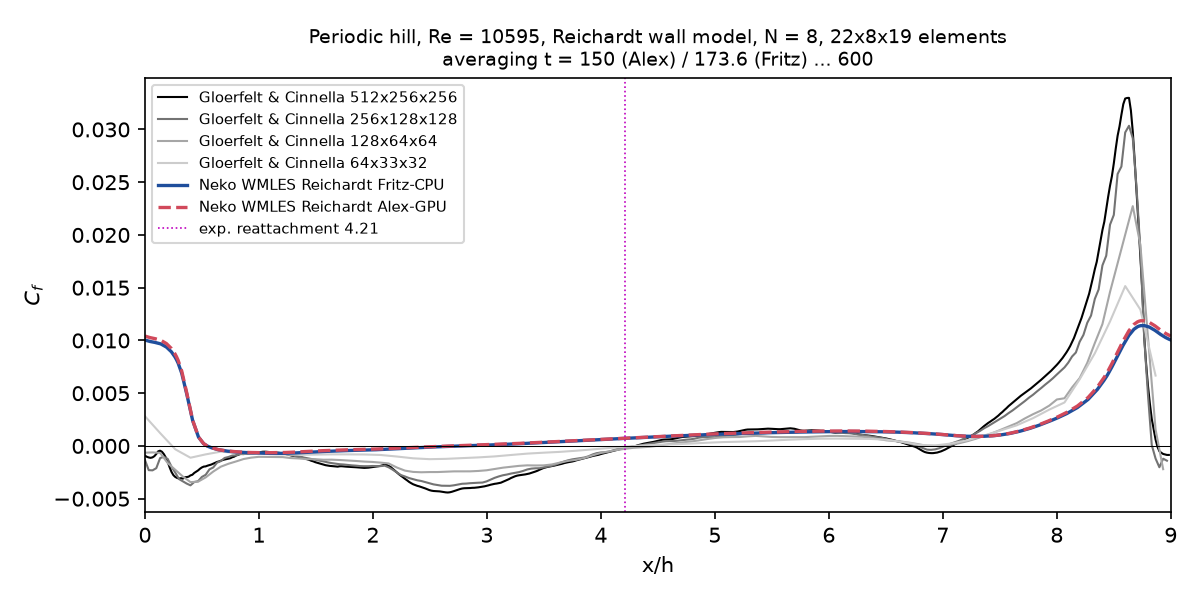
\includegraphics[width=0.85\textwidth]{figures/cf_bottom_Reichardt.png}
\caption{Skin friction on the hill wall: Neko WMLES with the Reichardt model
(reconstructed from the mean velocity at the sampling point) and the LES of
Gloerfelt \& Cinnella~\cite{gloerfelt2019} on four grids.}
\label{fig:hillcf}
\end{figure}

\subsection{Profiles}

Figures~\ref{fig:hillu}--\ref{fig:hilluv} compare the profiles with the
finest reference grid; Table~\ref{tab:hillprof} lists characteristic values.
At the wall, the Neko profiles show the slip velocity that the wall model
allows.

\begin{itemize}
  \item \textbf{Upper channel, and downstream from $x/h \approx 5$:} the
    mean velocity agrees well with the reference.
  \item \textbf{Bubble:} it starts with backflow of the right strength,
    $\langle u\rangle_{\min} = -0.17$ at $x/h = 1$ and $-0.21$ at $x/h = 2$,
    against $-0.13$ and $-0.25$ in the reference. It then closes early: at
    $x/h = 3$ the backflow is almost gone ($-0.02$ against $-0.14$), and at
    $x/h = 4$ the flow near the wall is forward.
  \item \textbf{Turbulence:} in the early shear layer at $x/h = 1$ and 2,
    $\langle u'u'\rangle$ and $-\langle u'v'\rangle$ are 15--35\,\% higher
    than in the reference; at $x/h = 0.5$ the excess is 0--15\,\%.
    Downstream of reattachment ($x/h \ge 4$) they are up to 15\,\% lower.
  \item \textbf{Crest ($x/h = 0.05$):} the fine reference grids show the
    shear layer starting at the wall, with $\langle u'u'\rangle$ up to 0.12.
    In the Neko runs the flow there is still attached, and the near-wall
    fluctuations stay at 0.03.
\end{itemize}

\begin{table}[htbp]
\centering
\small
\caption{Minimum of $\langle u\rangle$ and maxima of the Reynolds stresses
along the stations. Neko: Fritz / Alex, full averaging range. Reference:
Gloerfelt \& Cinnella, $512\times256\times256$.}
\label{tab:hillprof}
\begin{tabular}{@{}ccccccc@{}}
\toprule
$x/h$ & \multicolumn{2}{c}{$\langle u\rangle_{\min}$} &
\multicolumn{2}{c}{$\langle u'u'\rangle_{\max}$} &
\multicolumn{2}{c}{$-\langle u'v'\rangle_{\max}$} \\
 & Neko & ref. & Neko & ref. & Neko & ref. \\
\midrule
0.5 & $-0.067$ / $-0.064$ & $-0.080$ & 0.119 / 0.128 & 0.112 & 0.042 / 0.045 & 0.042 \\
1 & $-0.174$ / $-0.168$ & $-0.135$ & 0.109 / 0.120 & 0.093 & 0.052 / 0.056 & 0.042 \\
2 & $-0.213$ / $-0.194$ & $-0.253$ & 0.101 / 0.114 & 0.087 & 0.043 / 0.047 & 0.036 \\
3 & $-0.025$ / $-0.013$ & $-0.140$ & 0.090 / 0.100 & 0.091 & 0.034 / 0.037 & 0.035 \\
4 & slip $>0$ & $-0.005$ & 0.071 / 0.078 & 0.079 & 0.026 / 0.027 & 0.030 \\
6 & slip $>0$ & 0.000 & 0.048 / 0.050 & 0.055 & 0.017 / 0.017 & 0.020 \\
\bottomrule
\end{tabular}
\end{table}

\begin{figure}[htbp]
\centering
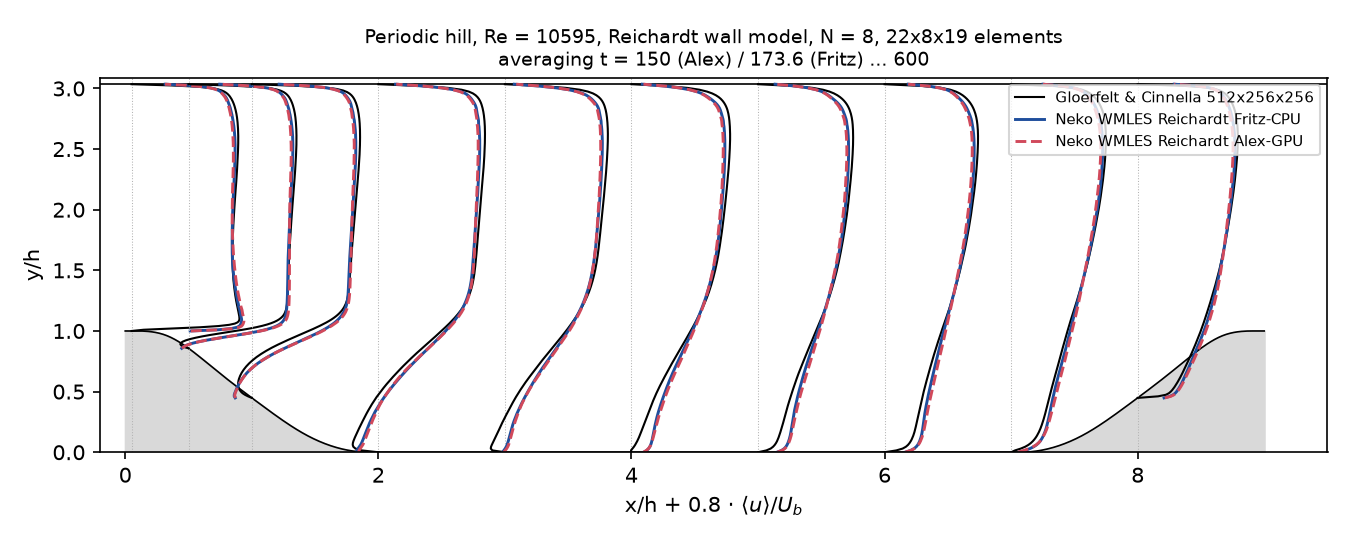
\includegraphics[width=\textwidth]{figures/profiles_u_Reichardt.png}\\[1ex]
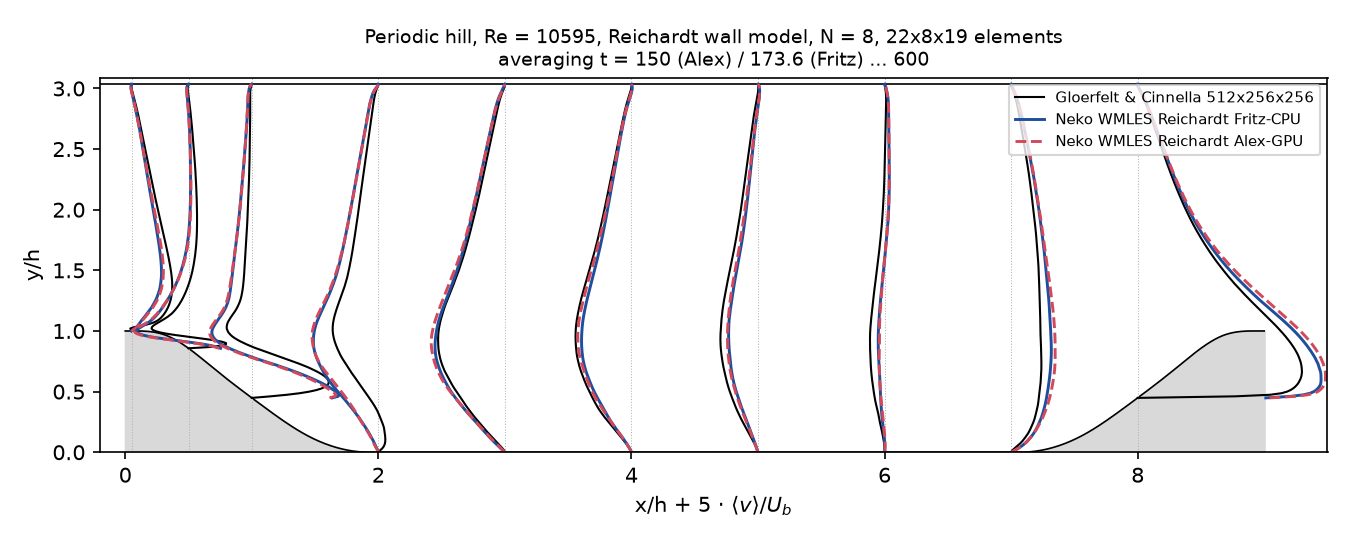
\includegraphics[width=\textwidth]{figures/profiles_v_Reichardt.png}
\caption{Mean velocity $\langle u\rangle$ (top) and $\langle v\rangle$
(bottom), Reichardt model, against Gloerfelt \&
Cinnella~\cite{gloerfelt2019}, $512\times256\times256$.}
\label{fig:hillu}
\end{figure}

\begin{figure}[htbp]
\centering
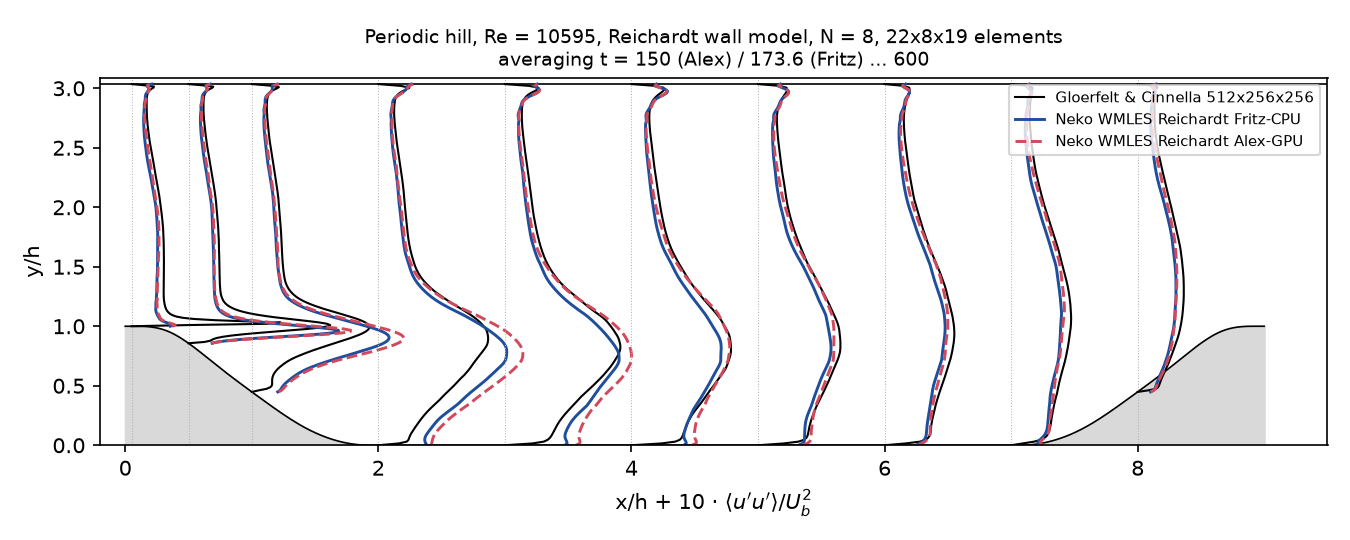
\includegraphics[width=\textwidth]{figures/profiles_upup_Reichardt.png}\\[1ex]
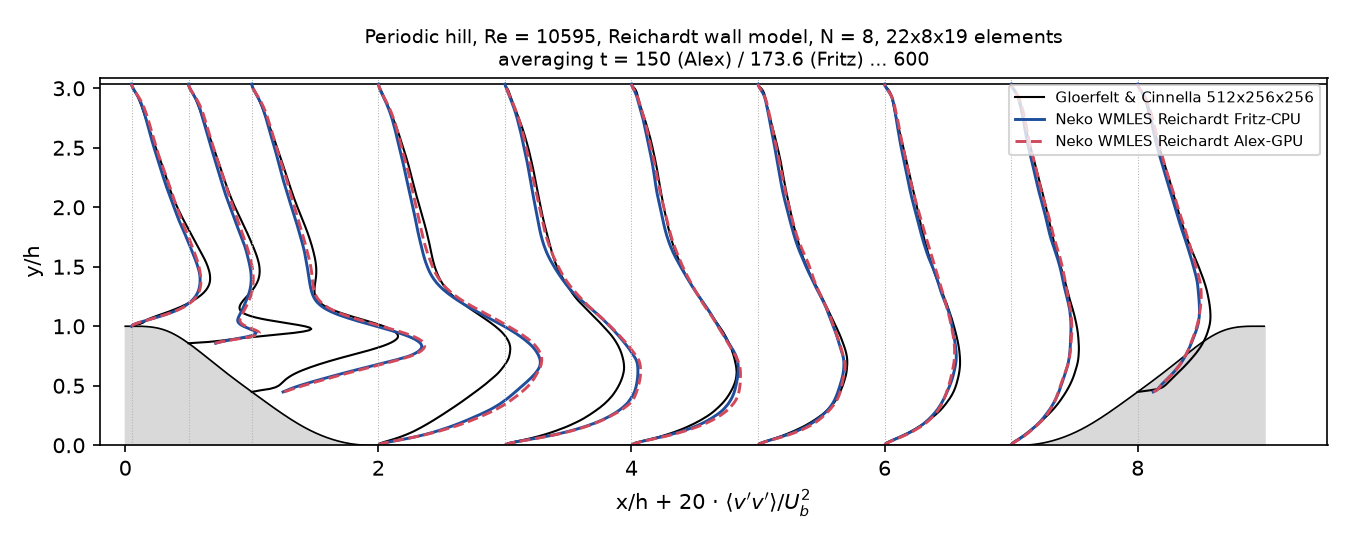
\includegraphics[width=\textwidth]{figures/profiles_vpvp_Reichardt.png}\\[1ex]
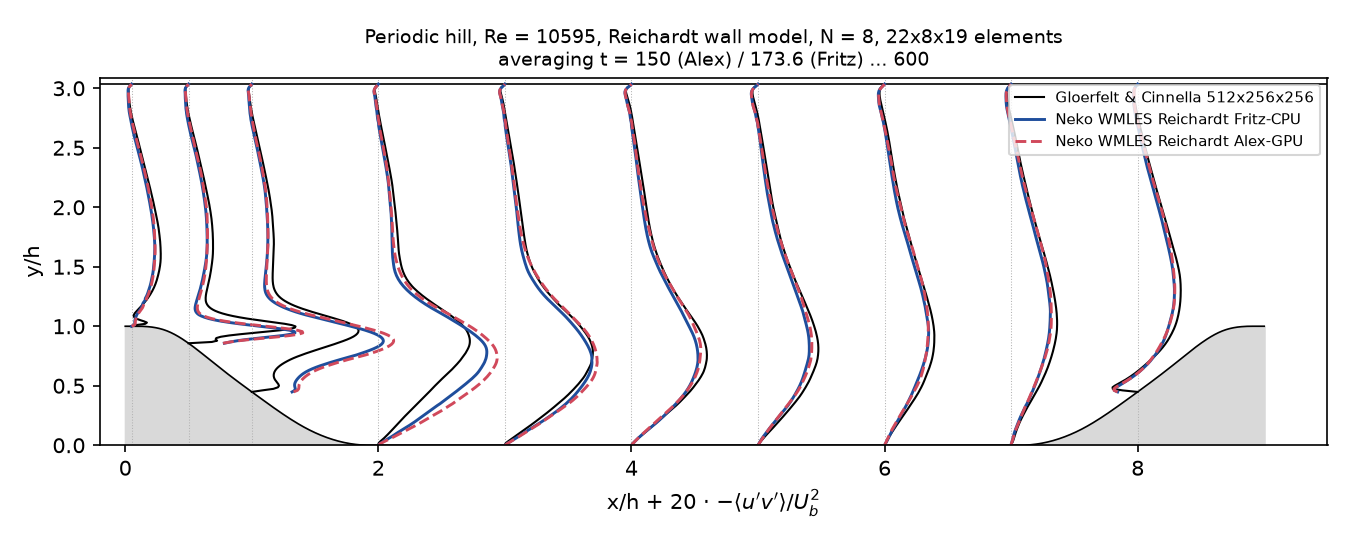
\includegraphics[width=\textwidth]{figures/profiles_upvp_Reichardt.png}
\caption{Reynolds stresses $\langle u'u'\rangle$, $\langle v'v'\rangle$ and
$-\langle u'v'\rangle$, Reichardt model, against Gloerfelt \&
Cinnella~\cite{gloerfelt2019}, $512\times256\times256$.}
\label{fig:hilluv}
\end{figure}

\subsection{Discussion}

The main deficiency is the separation over the crest. Separation there is
driven by the adverse pressure gradient on the lee side of the hill.
Reichardt's law is an equilibrium law without a pressure-gradient term: as
long as the velocity at the sampling point is directed downstream, the model
returns a positive, here large, wall shear stress. The delayed separation at
$x/h \approx 0.55$, the attached crest with $C_f \approx 0.009\ldots0.010$
and the low
fluctuations at $x/h = 0.05$ are consistent with this. A shorter bubble
follows. A second factor is resolution: with 8 elements over the height, the
crest region and the early shear layer are coarse. Gloerfelt \& Cinnella
identify exactly this region as the most sensitive one for the whole
solution.

Two next steps follow directly:
\begin{itemize}
  \item The Duprat model in \code{local} mode, which is designed for
    pressure-gradient effects, on the same mesh and with the same
    evaluation. It was tested in the original paper~\cite{duprat2011} on
    this flow.
  \item A mesh with more elements, or stronger clustering, in the wall-normal
    direction near the crest, to separate the model effect from the
    resolution effect.
\end{itemize}

\subsection{GPU (Alex) versus CPU (Fritz)}
\label{sec:gpucpu}

For a like-for-like comparison, both runs were evaluated over the same
windows, $t = 200\ldots600$: eight windows of 50 time units.

\begin{itemize}
  \item \textbf{Agreement:} the mean velocity and $C_f$ agree closely. The
    separation point is the same (0.547 against 0.546). The reattachment
    points agree within their scatter: $2.71 \pm 0.03$ on Alex and
    $2.78 \pm 0.08$ on Fritz, 0.9$\sigma$ apart.
  \item \textbf{Forces:} they differ by 2--6\,\% at 1.6--2.3$\sigma$.
    On the hill wall, $F_{x,p}$ is $+4.1\,\%$ and $F_{x,v}$ $+5.5\,\%$ on
    the GPU; on the top wall, $F_{x,v}$ is $-2.4\,\%$. The forcing
    $\langle f\rangle$ is $+3.5\,\%$, at 1.8$\sigma$.
  \item \textbf{Turbulence in the shear layer:} here the GPU run is
    systematically higher. At $x/h = 0.5\ldots4$ the peaks of
    $\langle u'u'\rangle$ are 8--13\,\% higher, at 1.9--3.1$\sigma$, and
    those of $-\langle u'v'\rangle$ 5--10\,\% higher. 16 of 18 peak values
    of $\langle u'u'\rangle$, $\langle v'v'\rangle$ and
    $-\langle u'v'\rangle$ at $x/h = 0.5, 1, 2, 3, 4, 6$ are higher on the
    GPU. At $x/h = 6$ the difference has vanished (full table in
    \code{results\_Re10595\_reichardt/common/gpu\_cpu\_windows.txt}).
\end{itemize}

The consistent sign first suggested a systematic difference between the CUDA
and the CPU code path in a device-specific part of the solver:
\begin{itemize}
  \item the LES model;
  \item the gradient jump penalty;
  \item the dealiased advection.
\end{itemize}

The Duprat runs (Section~\ref{sec:hilldup-gpucpu}) speak against this. They
used the same two builds, so the same solver code on both machines, and show
no such pattern. A solver-level code-path difference is therefore unlikely.
Two explanations remain:
\begin{itemize}
  \item a fluctuation that the window statistics underestimate. The 18 peak
    values come from the same eight windows and are correlated, so
    ``16 of 18'' overstates the significance;
  \item something specific to the Reichardt kernels, although the runs agree
    near the wall, where the wall model acts.
\end{itemize}

Statistics cannot settle this; a deterministic test can. Both machines
restart from the same checkpoint with a fixed $\Delta t$ and write the forces
every step for about 20 steps. Identical algorithms give differences at
round-off level, like a CPU run with a different rank count. A code-path
difference shows from the first step on. The case file, a comparison script
and instructions are in \code{periodic\_hill/gpu\_cpu\_check}. The GPU
warning was nevertheless removed after the Duprat comparison
(Section~\ref{sec:hilldup-gpucpu}); the test remains useful as a check.

An attempt to run the same comparison in the container with the OpenCL
backend (PoCL on the CPU) did not get that far. The OpenCL run produced NaN
in the first pressure solve, even without wall model, GJP and LES model. The
OpenCL channel case had run before, so this concerns the PoCL test
environment with this case, not CUDA, and was not pursued further.

\subsection{Performance}

On one Alex GPU a time step took 0.051~s (median), on a full Fritz node with
72 ranks 0.403~s, a factor of about 8. Both runs used
$\Delta t \approx 3.35\cdot10^{-3}$ at a mean CFL of 0.48--0.49. By the total
elapsed times in the logs, the GPU run needed 2.2~hours for 500 time units and
the Fritz run 14.6~hours for 426 time units.

%=====================================================================
\section{Periodic hill at $Re_h = 10\,595$ with the Duprat model}
\label{sec:hilldup}
%=====================================================================

\subsection{Case and runs}

The case is the one of Section~\ref{sec:hill}. Mesh, numerics, forcing and
output are the same; only the wall model differs:
\begin{itemize}
  \item \textbf{Wall model:} Duprat on both walls with $\kappa = 0.41$,
    $\beta = 0.78$ and $A = 17$, sampling at GLL index~3. The pressure
    gradient is evaluated locally (\code{"type": "local"}) with
    \code{filter\_time}~1.0 and \code{start\_time}~50.
  \item \textbf{Additional output:} \code{user\_stats} of the registry fields
    \code{tau}, \code{duprat\_dpds} and \code{duprat\_alpha}, averaged over
    $z$ from $t = 150$. This gives $\langle|\tau_w|\rangle$, the filtered
    $\dpds$ seen by the model, and $\alpha$ along both walls.
\end{itemize}

\noindent Both runs reached $t = 600$. They used the same two builds as the
Reichardt runs, so the solver code on each machine is the same for both
models.

\begin{center}
\small
\begin{tabularx}{\textwidth}{@{}lX@{}}
\toprule
Run & Set-up \\
\midrule
Fritz (CPU) & Intel build, 72 ranks. The first job reached the 24-hour limit
at $t = 493.8$, after its last checkpoint at $t = 483.394$. The second job
restarted from that checkpoint. The statistics therefore cover
$t = 150\ldots450$ and $483.4\ldots600$, 46 flow-through times. The window
$450\ldots483.4$ was lost because its output at $t = 500$ was never
written. The logs of both jobs are joined at the restart. The filtered
$\dpds$ is not in the checkpoint and builds up again within about one
\code{filter\_time} after the restart. \\
Alex (GPU) & GNU build, CUDA, one GPU, from $t = 0$; statistics
$t = 150\ldots600$, 50 flow-through times. \\
\bottomrule
\end{tabularx}
\end{center}

\noindent The evaluation uses the scripts and the $C_f$ reconstruction of
Section~\ref{sec:hill}, now with the Duprat law and the mean filtered $\dpds$.
For the Fritz run, \code{ph\_stats.py} takes one start time per output series
(150 and 483.394), and \code{ph\_forces.py} uses each log only up to the start
of the next. The results are in
\code{periodic\_hill/analysis/results\_Re10595\_duprat}.

\subsection{Forces}

\begin{table}[htbp]
\centering
\footnotesize
\setlength{\tabcolsep}{4pt}
\caption{Time-averaged forces, scaled with $2/(\rho U_b^2 L_x L_z)$, and the
flow-rate forcing $f$ for both models. Full averaging range of each run;
$\pm$ standard error over windows of 50 time units. The Reichardt columns
repeat Table~\ref{tab:hillforces}.}
\label{tab:hilldupforces}
\begin{tabular}{@{}lcccc@{}}
\toprule
 & \multicolumn{2}{c}{Duprat} & \multicolumn{2}{c}{Reichardt} \\
 & Fritz (CPU) & Alex (GPU) & Fritz (CPU) & Alex (GPU) \\
\midrule
hill wall, $F_{x,p}$ & $0.0622 \pm 0.0009$ & $0.0595 \pm 0.0012$ & $0.0434 \pm 0.0009$ & $0.0449 \pm 0.0005$ \\
hill wall, $F_{x,v}$ & $0.00285 \pm 0.00009$ & $0.00286 \pm 0.00012$ & $0.00202 \pm 0.00006$ & $0.00212 \pm 0.00003$ \\
top wall, $F_{x,v}$ & $0.00854 \pm 0.00006$ & $0.00859 \pm 0.00006$ & $0.00616 \pm 0.00006$ & $0.00605 \pm 0.00004$ \\
mean $C_f$ from $\langle|\tau_w|\rangle$, hill/top & 0.00284 / 0.00803 & 0.00284 / 0.00805 & -- & -- \\
reconstr.\ mean $C_f$, hill/top & 0.00236 / 0.00774 & 0.00236 / 0.00778 & 0.00169 / 0.00566 & 0.00176 / 0.00555 \\
forcing $\langle f\rangle$ & 0.01291 & 0.01243 & 0.00906 & 0.00932 \\
balance & 1.010 & 1.010 & 1.009 & 1.008 \\
\bottomrule
\end{tabular}
\end{table}

\begin{itemize}
  \item \textbf{Compared with Reichardt} (same machine): the pressure drag
    on the hill is 33--43\,\% higher, and the skin friction on both walls
    35--42\,\% higher. The forcing that keeps $U_b = 1$ rises by 33--42\,\%.
    The momentum balance again closes to within 1\,\%.
  \item \textbf{Wall shear stress statistic:} the mean of the model's
    $|\tau_w|$, with the sign of the mean flow, matches the
    \code{force\_torque} skin friction of the hill wall to 0.4\,\%
    (0.00284 against 0.00285). On the top wall it is 6\,\% lower.
  \item \textbf{Law against flow:} the source of the higher friction can be
    separated by applying both laws to the same mean flow of the Duprat
    runs:
    \begin{itemize}
      \item On the hill wall the Duprat law gives twice the mean $C_f$ of the
        Reichardt law (0.00236 against 0.00113). Most of the difference
        comes from the windward face.
      \item On the top wall the Duprat law gives 25\,\% more (0.0077 against
        0.0062), although $\alpha$ is at least 0.91 there (mean 0.95). The
        remaining 12\,\% come from the flow: the velocity at the top sampling
        points is about 7\,\% higher than in the Reichardt runs.
    \end{itemize}
  \item \textbf{Against the reference:} the mean $C_f$ of the hill wall,
    0.0024--0.0029, is about twice that of the finest grid of Gloerfelt \&
    Cinnella (0.00132). With Reichardt it was 0.0017--0.0021.
\end{itemize}

\begin{figure}[htbp]
\centering
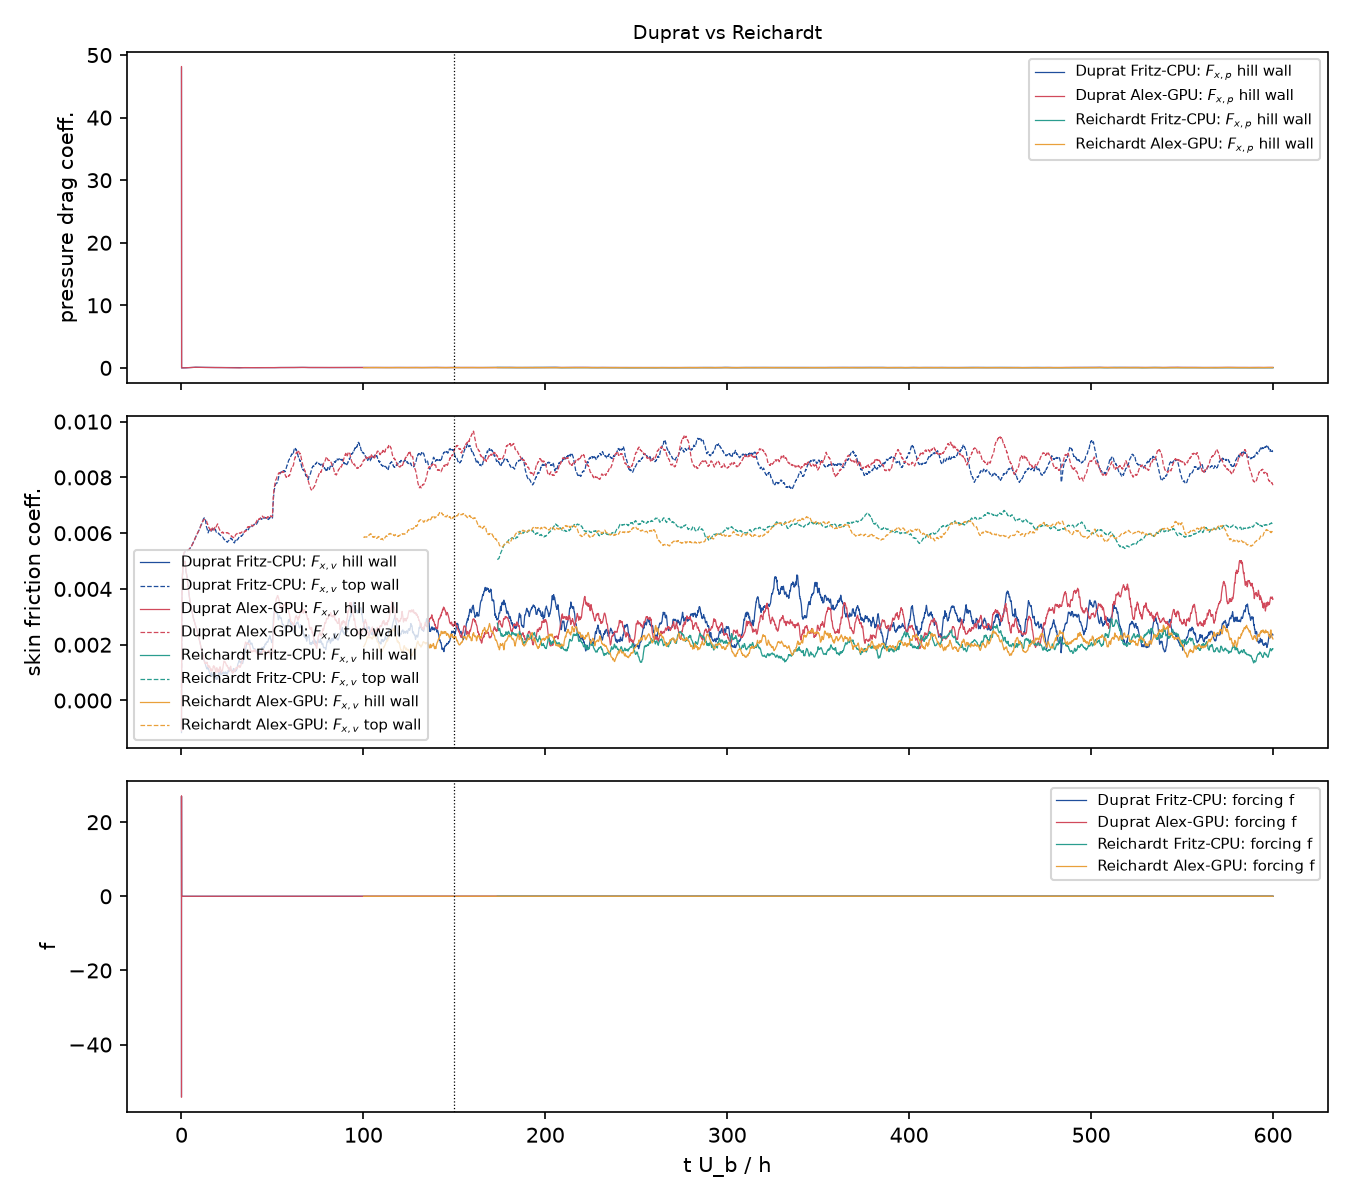
\includegraphics[width=0.85\textwidth]{figures/forces_time_Duprat_vs_Reichardt.png}
\caption{Forces and forcing over time for both models, Fritz (CPU) and Alex
(GPU).}
\label{fig:hilldupforces}
\end{figure}

\subsection{Skin friction, separation and reattachment}

\begin{table}[htbp]
\centering
\footnotesize
\setlength{\tabcolsep}{4pt}
\caption{Zero crossings and extrema of $C_f$ on the hill wall. Neko:
reconstructed $C_f$; in parentheses, the mean reattachment point over the
output windows with its standard error, and the bubble minimum from
$\langle|\tau_w|\rangle$. Reference values as in Table~\ref{tab:hillsep}.}
\label{tab:hilldupsep}
\begin{tabular}{@{}lcccc@{}}
\toprule
 & separation & reattachment & $C_{f,\min}$ (bubble) & $C_{f,\max}$ (windward) \\
\midrule
Neko Duprat, Fritz (CPU) & 0.45 & 3.33 ($3.37 \pm 0.10$) & $-0.0015$ ($-0.0028$) & 0.031 \\
Neko Duprat, Alex (GPU) & 0.45 & 3.21 ($3.21 \pm 0.08$) & $-0.0013$ ($-0.0029$) & 0.031 \\
Neko Reichardt, Fritz (CPU) & 0.55 & 2.78 ($2.78 \pm 0.07$) & $-0.0007$ & 0.011 \\
Neko Reichardt, Alex (GPU) & 0.55 & 2.71 ($2.71 \pm 0.03$) & $-0.0006$ & 0.012 \\
Gloerfelt $512\times256\times256$ & $-0.12$ & 4.31 & $-0.0044$ & 0.033 \\
Gloerfelt $256\times128\times128$ & $-0.16$ & 4.32 & $-0.0038$ & 0.030 \\
Experiment (Rapp \& Manhart) & & 4.21 & & \\
\bottomrule
\end{tabular}
\end{table}

\begin{itemize}
  \item \textbf{Reattachment:} it moves downstream by about 0.5, from
    2.7--2.8 to 3.2--3.4. That is still about 1 short of the reference.
  \item \textbf{Separation:} it moves upstream from 0.55 to 0.45. The flow
    is still attached over the crest, where the reference separates at or
    just before it, but $C_f$ there drops from 0.010 to 0.007.
  \item \textbf{Bubble:} it is twice as strong as with Reichardt. The
    reconstruction gives $C_f \approx -0.0014$ and $\langle|\tau_w|\rangle$
    gives $-0.0028$, against $-0.0038\ldots-0.0044$ in the reference.
  \item \textbf{Windward peak:} $C_{f,\max} = 0.031$ at $x/h = 8.63$ now
    matches the fine reference grids (0.030--0.033). Reichardt gave 0.011.
    Here the strong favourable gradient on the windward face acts as the
    model intends.
  \item \textbf{Recovery region} ($x/h = 4\ldots7$): $C_f$ from
    $\langle|\tau_w|\rangle$ is about 0.002 and the reconstruction gives
    0.0007, against 0.0008 on average in the reference.
\end{itemize}

\begin{figure}[htbp]
\centering
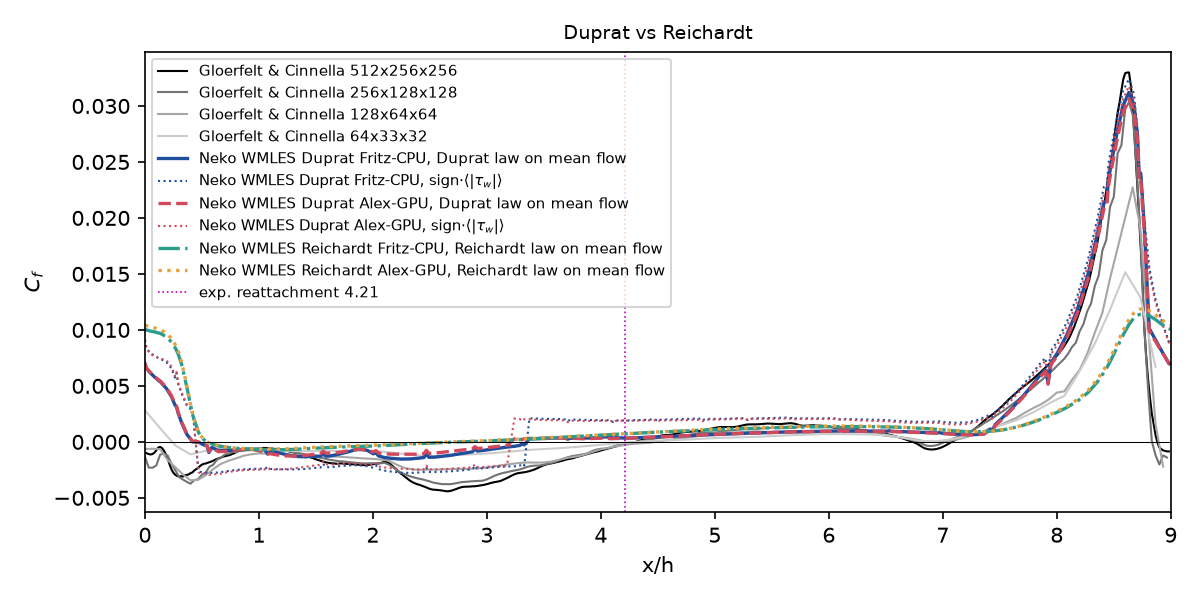
\includegraphics[width=0.85\textwidth]{figures/cf_bottom_Duprat_vs_Reichardt.png}
\caption{Skin friction on the hill wall: Neko WMLES with the Duprat model
(reconstructed with the Duprat law, solid and dashed; from
$\langle|\tau_w|\rangle$ with the sign of the mean flow, dotted) and with the
Reichardt model, against Gloerfelt \& Cinnella~\cite{gloerfelt2019}.}
\label{fig:hilldupcf}
\end{figure}

\subsection{Profiles}

\begin{table}[htbp]
\centering
\small
\caption{Minimum of $\langle u\rangle$ and maxima of the Reynolds stresses
along the stations. Neko: Fritz / Alex, full averaging range. Reference:
Gloerfelt \& Cinnella, $512\times256\times256$. ``slip'': the minimum is the
slip velocity at the wall, positive.}
\label{tab:hilldupprof}
\begin{tabular}{@{}cccccccc@{}}
\toprule
$x/h$ & \multicolumn{3}{c}{$\langle u\rangle_{\min}$} &
\multicolumn{2}{c}{$\langle u'u'\rangle_{\max}$} &
\multicolumn{2}{c}{$-\langle u'v'\rangle_{\max}$} \\
 & Duprat & Reichardt & ref. & Duprat & ref. & Duprat & ref. \\
\midrule
0.5 & $-0.112$ / $-0.111$ & $-0.067$ / $-0.064$ & $-0.080$ & 0.129 / 0.127 & 0.112 & 0.046 / 0.047 & 0.042 \\
1 & $-0.149$ / $-0.137$ & $-0.174$ / $-0.168$ & $-0.135$ & 0.110 / 0.108 & 0.093 & 0.051 / 0.052 & 0.042 \\
2 & $-0.237$ / $-0.197$ & $-0.213$ / $-0.194$ & $-0.253$ & 0.104 / 0.103 & 0.087 & 0.046 / 0.044 & 0.036 \\
3 & $-0.115$ / $-0.084$ & $-0.025$ / $-0.013$ & $-0.140$ & 0.100 / 0.099 & 0.091 & 0.041 / 0.039 & 0.035 \\
4 & slip & slip & $-0.005$ & 0.086 / 0.087 & 0.079 & 0.034 / 0.033 & 0.030 \\
6 & slip & slip & 0.000 & 0.064 / 0.064 & 0.055 & 0.023 / 0.022 & 0.020 \\
\bottomrule
\end{tabular}
\end{table}

\begin{itemize}
  \item \textbf{Mean velocity} (Table~\ref{tab:hilldupprof},
    Figure~\ref{fig:hilldupu}):
    \begin{itemize}
      \item The largest gain is at $x/h = 3$: the backflow is $-0.08$ to
        $-0.12$, against $-0.14$ in the reference and only $-0.01$ to
        $-0.03$ with Reichardt.
      \item At $x/h = 2$ the backflow is close to the reference on the CPU
        ($-0.24$ against $-0.25$) and 20\,\% weaker on the GPU.
      \item At $x/h = 0.5$ it is too strong, $-0.11$ against $-0.08$.
    \end{itemize}
  \item \textbf{Turbulence:}
    \begin{itemize}
      \item In the shear layer at $x/h = 1$ and 2, the peaks of
        $\langle u'u'\rangle$ and $-\langle u'v'\rangle$ are 15--30\,\% above
        the reference, as with Reichardt.
      \item Downstream of reattachment ($x/h \ge 4$) they are now 9--16\,\%
        above the reference. With Reichardt they were up to 15\,\% below.
    \end{itemize}
\end{itemize}

\begin{figure}[htbp]
\centering
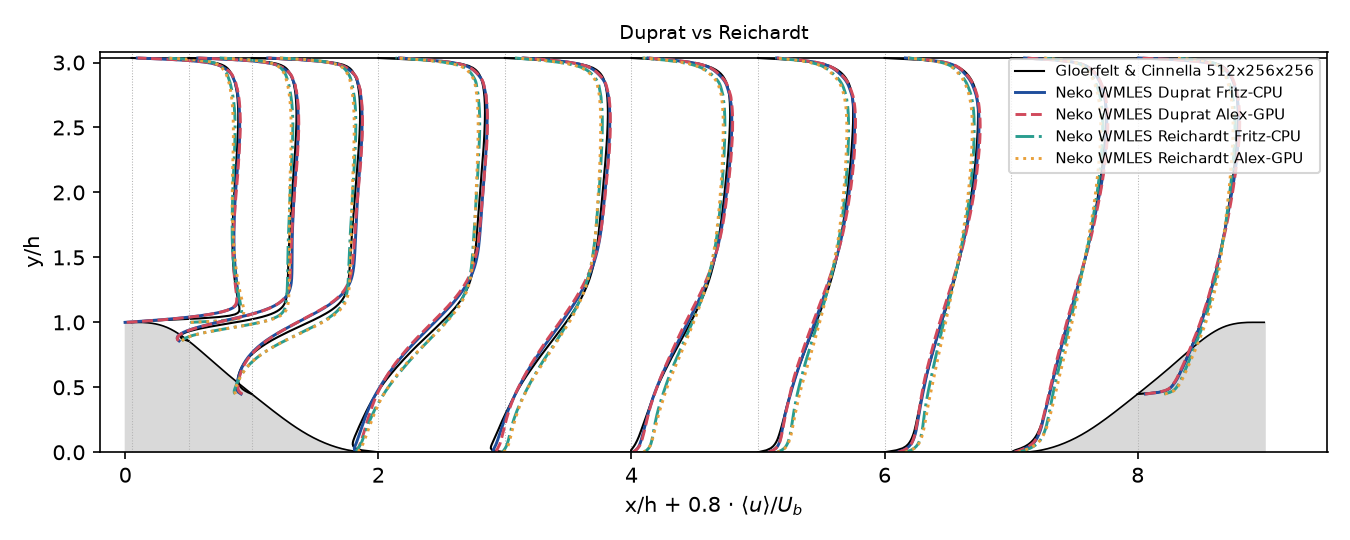
\includegraphics[width=\textwidth]{figures/profiles_u_Duprat_vs_Reichardt.png}\\[1ex]
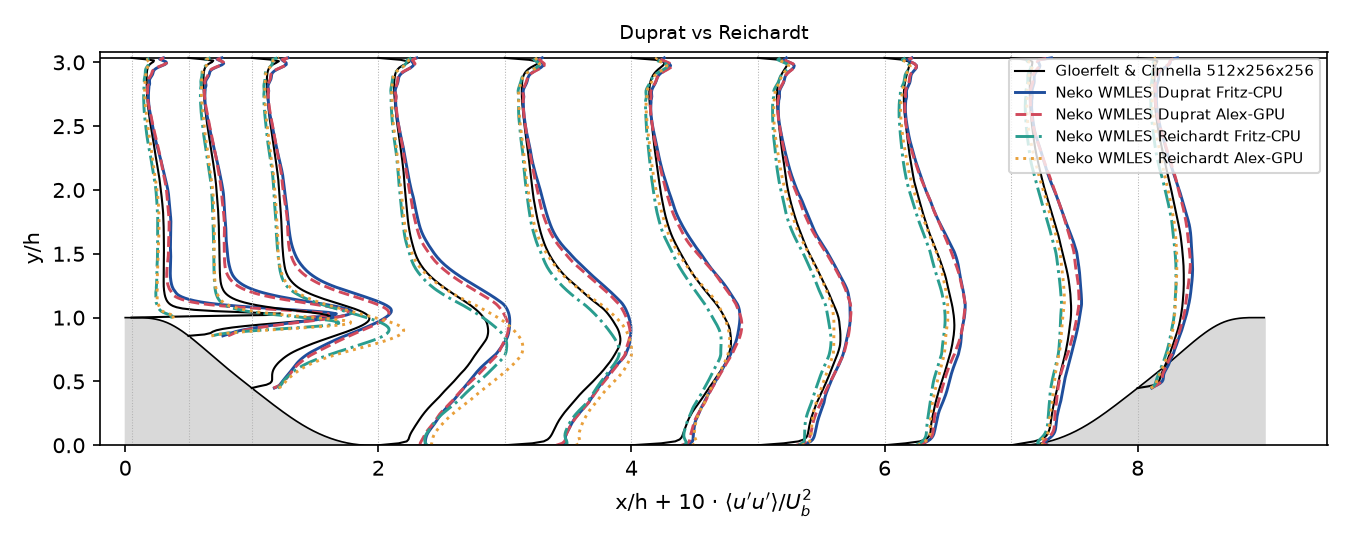
\includegraphics[width=\textwidth]{figures/profiles_upup_Duprat_vs_Reichardt.png}\\[1ex]
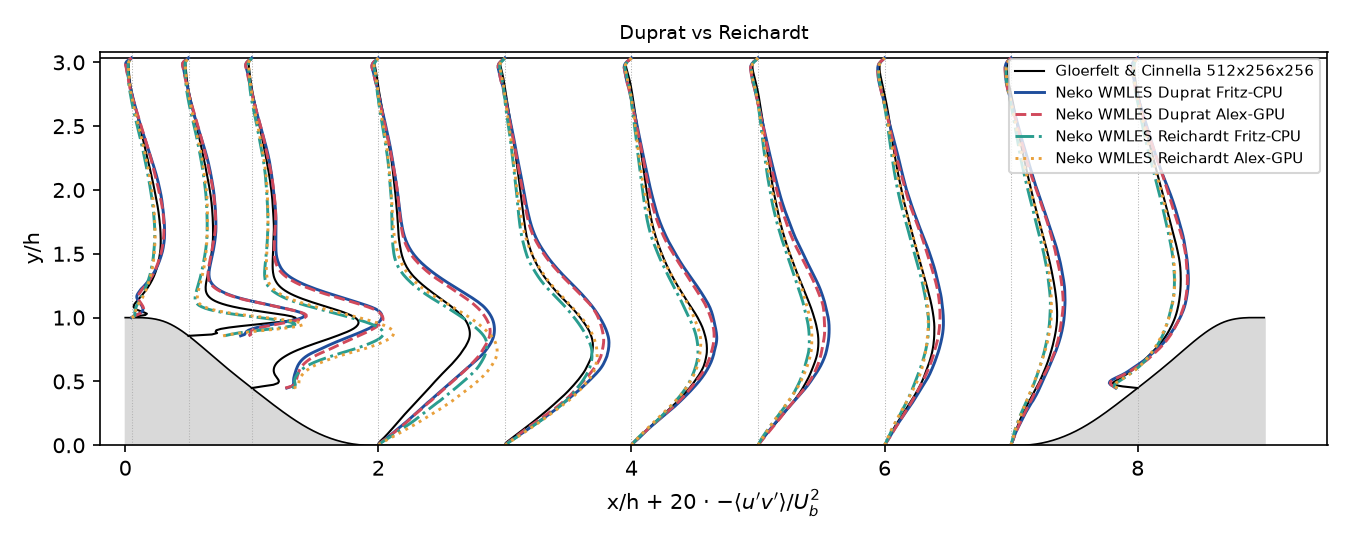
\includegraphics[width=\textwidth]{figures/profiles_upvp_Duprat_vs_Reichardt.png}
\caption{Mean velocity $\langle u\rangle$, $\langle u'u'\rangle$ and
$-\langle u'v'\rangle$ for both models and both machines, against Gloerfelt
\& Cinnella~\cite{gloerfelt2019}, $512\times256\times256$.}
\label{fig:hilldupu}
\end{figure}

\subsection{The pressure gradient seen by the model}
\label{sec:hilldup-dpds}

Figure~\ref{fig:hilldupwall} shows the mean $\alpha$ and the mean filtered
$\dpds$ along the hill wall. Table~\ref{tab:hilldupdpds} compares the
filtered $\dpds$ with the gradient of the mean pressure. Both are taken at
the sampling points, and both are signed with respect to the local mean flow
direction, so they are comparable.

\begin{table}[htbp]
\centering
\small
\caption{Range of the mean filtered $\dpds$ used by the model and of the
gradient of the mean pressure along the hill wall, at the sampling points.
Positive values are adverse to the mean flow at the sampling point. Fritz
(CPU); the Alex values agree to within a few per cent.}
\label{tab:hilldupdpds}
\begin{tabular}{@{}lcc@{}}
\toprule
region ($x/h$) & model, $\langle\dpds\rangle_\mathrm{filt}$ & mean pressure, $\partial\langle p\rangle/\partial s$ \\
\midrule
crest, 0--0.4 & $+0.011\ldots+0.146$ & $+0.014\ldots+0.248$ \\
bubble, 0.5--3 (backflow) & $-0.012\ldots+0.004$ & $-0.122\ldots-0.024$ \\
recovery, 4--7 & $-0.001\ldots+0.016$ & $+0.035\ldots+0.061$ \\
windward face, 8.3--8.8 & $-0.578\ldots-0.143$ & $-0.858\ldots-0.200$ \\
\bottomrule
\end{tabular}
\end{table}

\begin{itemize}
  \item \textbf{Strength:} averaged over each region, the model sees about
    two thirds of the mean gradient on the windward face and a little more
    than half at the crest. In the bubble it sees only 1/13 of it, and in the
    recovery region 1/8 to 1/9. CPU and GPU agree.
  \item \textbf{Cause:} the gradient is projected on the
    \emph{instantaneous} wall-parallel velocity and limited to the Stokes
    bound before it is filtered (Section~\ref{sec:local}). Where the flow
    direction changes often, as in the bubble and near reattachment, the
    projections cancel in the time filter, and the limit cuts the peaks.
  \item \textbf{Element boundaries:} $\alpha$ shows narrow spikes there, and
    $|\dpds|$ dips to about half of its neighbours. They appear identically
    on CPU and GPU, so they are not a device effect. The most likely cause is
    the one-sided pressure gradient at the element faces together with the
    Stokes limit.
\end{itemize}

\begin{figure}[htbp]
\centering
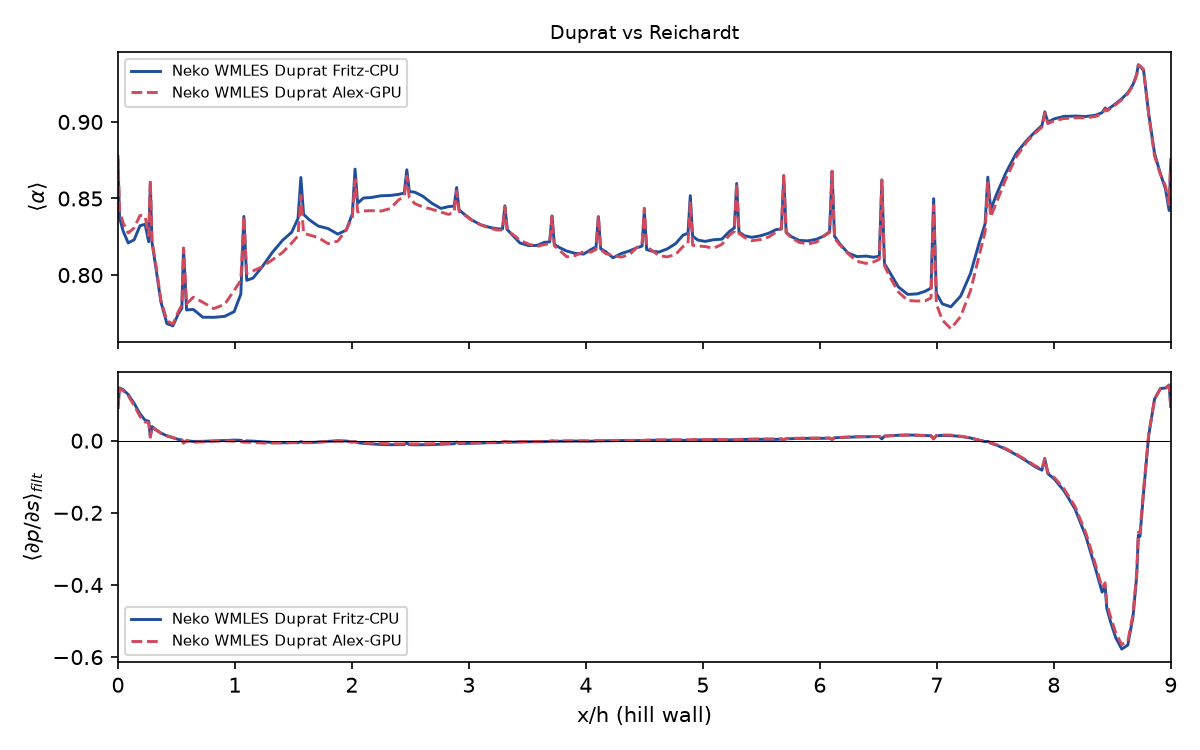
\includegraphics[width=0.85\textwidth]{figures/wall_alpha_dpds_Duprat_vs_Reichardt.png}
\caption{Mean $\alpha = \utau^2/\utp^2$ (top) and mean filtered $\dpds$
(bottom) along the hill wall, Duprat model, Fritz (CPU) and Alex (GPU).}
\label{fig:hilldupwall}
\end{figure}

\subsection{GPU (Alex) versus CPU (Fritz)}
\label{sec:hilldup-gpucpu}

The comparison uses all output windows of 50 time units: eight on Fritz and
nine on Alex. The table is in
\code{results\_Re10595\_duprat/gpu\_cpu\_windows\_duprat.txt}, made with the
new script \code{gpu\_cpu\_windows.py}. Run on the Reichardt data, the script
reproduces the table of Section~\ref{sec:gpucpu} exactly.

\begin{itemize}
  \item \textbf{Mean flow and skin friction:}
    \begin{itemize}
      \item The separation point is the same, 0.446 against 0.451.
      \item The reattachment points over the windows are $3.37 \pm 0.10$ on
        the CPU and $3.21 \pm 0.08$ on the GPU, 1.2$\sigma$ apart.
      \item $C_f$, $\alpha$ and $\dpds$ lie on top of each other
        (Figures~\ref{fig:hilldupcf} and~\ref{fig:hilldupwall}).
    \end{itemize}
  \item \textbf{Forces:}
    \begin{itemize}
      \item The skin friction agrees within 0.6\,\% on both walls.
      \item The pressure drag is 4.5\,\% and the forcing 3.8\,\% lower on
        the GPU, at 1.7--1.8$\sigma$. With Reichardt, both were about 4\,\%
        \emph{higher} on the GPU, at similar significance.
    \end{itemize}
  \item \textbf{Turbulence:} no systematic difference. Only 4 of the 18
    peak values are higher on the GPU. The differences are $-5.5$ to
    $+2.6\,\%$, all within 1.3$\sigma$.
  \item \textbf{Largest difference:} the backflow at $x/h = 2$, $-0.240$ on
    the CPU against $-0.199$ on the GPU (3.4$\sigma$). The CPU bubble is
    slightly stronger, which fits its later reattachment.
\end{itemize}

\noindent Two conclusions follow:
\begin{itemize}
  \item \textbf{No systematic difference:} there is no sign of a systematic
    difference between the CUDA and the CPU code path. Both models used the
    same builds on each machine, so this also argues against a solver-level
    cause of the Reichardt observation (Section~\ref{sec:gpucpu}).
  \item \textbf{Uncertainties too small:} both comparisons show 2--3$\sigma$
    differences, but in different quantities and with different signs.
    Standard errors over 50-unit windows therefore underestimate the
    run-to-run scatter of this flow, presumably because of slow modulations
    of the bubble.
\end{itemize}

\noindent On this basis the GPU warnings of both models were removed. The
deterministic restart test of Section~\ref{sec:gpucpu} remains the clean way
to confirm that the code paths agree.

\subsection{Performance}

\begin{itemize}
  \item \textbf{Cost per step:} 0.551~s on Fritz and 0.061~s on Alex
    (median). That is 37\,\% and 20\,\% more than with Reichardt.
  \item \textbf{Time step:} $\Delta t$ is 3--6\,\% smaller,
    $3.16\cdot10^{-3}$ and $3.23\cdot10^{-3}$.
  \item \textbf{Elapsed time:} the Fritz jobs took 23.9 and 5.7 hours, about
    174~s per time unit against 123~s with Reichardt. The Alex run took
    3.2 hours for 600 time units.
  \item \textbf{Likely cause} (not profiled): $U^*$ is evaluated by
    quadrature inside the Newton iteration, and only on the ranks that own
    wall elements. On the CPU this also unbalances the load.
\end{itemize}

\subsection{Discussion}

The Duprat model improves the hill flow where the pressure gradient is
strong and acts as the model intends:
\begin{itemize}
  \item the windward skin-friction peak;
  \item the earlier separation;
  \item a stronger and longer bubble, with reattachment 0.5 further
    downstream.
\end{itemize}
The reattachment is still about 1 short of the reference, and the friction
is too high.

The analysis of the pressure gradient explains much of this. In the bubble
and in the recovery region, the model sees only a fraction of the mean
pressure gradient (Section~\ref{sec:hilldup-dpds}). It is therefore closer
to an equilibrium model there than its formulation intends. Three changes to
the local mode follow; all keep the interface:
\begin{enumerate}
  \item Filter the gradient \emph{vector} first, then project it on the
    filtered flow direction and apply the limit. This avoids the cancellation
    in reversing flow.
  \item Average $\nabla p$ continuously across element faces before
    sampling. This removes the dips at the element boundaries.
  \item Include the driving body force in the pressure gradient. On the
    hill it is $f \approx 0.012$: small on the windward face, but 20--35\,\%
    of the mean gradient in the recovery region.
\end{enumerate}
These changes can be tested on this case with the same evaluation.
Independently of the model, the coarse wall-normal resolution near the crest
(Section~\ref{sec:hill}) remains a factor.

%=====================================================================
\section{Test environment}
%=====================================================================

\begin{itemize}
  \item Cloud container: gfortran, MPICH, json-fortran 9.0.3 (built
    locally), Neko built with \code{-O1} on CPU and with
    \code{--with-opencl}. PoCL~5.0 (OpenCL on the CPU), with Neko's device
    selection patched from \code{CL\_DEVICE\_TYPE\_GPU} to
    \code{CL\_DEVICE\_TYPE\_ALL} in the test copy only.
  \item No \code{nvcc}, \code{hipcc}, Metal compiler, or GPU hardware.
  \item In this container, \code{mpirun -np 4} with MPICH started
    independent single-rank copies (Ubuntu's MPICH is built for PMIx, which
    Hydra does not serve), so the model comparisons used one rank. For the
    multi-rank tests of Section~\ref{sec:pr7}, OpenMPI~4.1.6 was installed
    and Neko built against it.
  \item With PoCL, the periodic hill produced NaN in the first pressure
    solve, even without wall model, GJP and LES model
    (Section~\ref{sec:gpucpu}).
  \item pFUnit~4.15.0 was built in the container. The unit suites of the
    upstream branches were run with gfortran~13.3 and OpenMPI~4.1.6, with the
    compiler flags of the upstream CI (\code{-g -O2 -pedantic -std=f2008}),
    in single and double precision.
  \item The ad-hoc test harnesses (kernel drivers, SciPy references, user
    files) lived in the session's scratch space and are not part of the
    repository. The kernel tests now live on as pFUnit suites; see the open
    items.
\end{itemize}

%=====================================================================
\section{Open items and recommendations}
\label{sec:open}
%=====================================================================

\begin{enumerate}
  \item \textbf{GPU validation:} both models have run the full hill on
    Alex (CUDA). Mean flow and skin friction agree with the CPU runs.
    \begin{itemize}
      \item The higher shear-layer turbulence of the Reichardt GPU run
        (Section~\ref{sec:gpucpu}) does not reappear with Duprat
        (Section~\ref{sec:hilldup-gpucpu}).
      \item The GPU warnings have been removed. The deterministic restart
        test in \code{periodic\_hill/gpu\_cpu\_check} would still settle the
        Reichardt observation.
    \end{itemize}
  \item \textbf{Duprat \code{local} mode:} the hill campaign is done
    (Section~\ref{sec:hilldup}). The model passes on too little of the
    pressure gradient where the flow reverses. Implement and test, on the
    same case with the same evaluation:
    \begin{itemize}
      \item filtering the gradient vector before the projection and the
        limit;
      \item averaging $\nabla p$ continuously across element faces;
      \item including the driving body force.
    \end{itemize}
    Also look at the cost: 37\,\% more per step than Reichardt on the
    CPU.
  \item \textbf{Wall-normal resolution of the hill mesh:} 8 elements over the
    height. A finer or more strongly clustered mesh near the crest would
    separate the wall-model effect from the resolution effect.
  \item \textbf{Mean wall shear stress as a statistic:} the Duprat runs
    average $|\tau_w|$ through \code{user\_stats}. On the hill wall this
    matches the \code{force\_torque} skin friction to 0.4\,\%. A signed
    streamwise $\tau_w$ would also resolve the bubble, where the mean of the
    magnitude overestimates $|C_f|$.
  \item \textbf{Thesis results:} confirm with D.~Bole which code version
    (with or without FIX~10) produced the hill results. Re-examine the
    Duprat hill results and the \code{h\_index}~=~7 channel result in light
    of Sections~\ref{sec:fix10} and \ref{sec:quadrature}.
  \item \textbf{Filter state in checkpoints:} the filtered $\dpds$ restarts
    from zero after a restart; it could be added to the checkpoint.
  \item \textbf{Normals at edge nodes:} let the wall-model base class use
    the projector's averaged normals (Section~\ref{sec:penetration}).
  \item \textbf{Permanent tests:} the upstream branches now carry pFUnit
    suites for the CPU kernels:
    \begin{itemize}
      \item Reichardt: 5 tests;
      \item Duprat: 8 tests, including the filter update.
    \end{itemize}
    Both pass in single and double precision with the CI flags, and so does
    the full unit suite. An integration test is still missing.
  \item \textbf{Documentation:} the user guide stated that
    \code{shear\_stress} and \code{wall\_model} only work with axis-aligned
    boundaries. In current Neko both require \code{full\_stress\_formulation},
    and the coupled projector constrains the normal velocity along the
    resolved node normal, as the hill tests confirm. The Duprat branch
    corrects the user guide and the comment in \code{wall\_model\_bc.f90}.
  \item \textbf{Upstream:} both models are on branches based on
    ExtremeFLOW/neko \code{develop}, \code{feature/reichardt-wall-model} and
    \code{feature/duprat-wall-model}. The Reichardt PR is open. The two PRs
    register their model in the same lists, so the second one to be merged
    needs a merge of \code{develop}, and \code{WALLM\_KNOWN\_TYPES} then has
    7 entries.
\end{enumerate}

%=====================================================================
\appendix
\section{Case-file examples}
%=====================================================================

\paragraph{Reichardt} (constants optional, shown with defaults):
\begin{lstlisting}[language=json]
{ "type": "wall_model", "zone_indices": [3, 4], "model": "reichardt",
  "kappa": 0.41, "C": 7.8, "B1": 11.0, "B2": 3.0,
  "sampling": { "type": "gll", "value": 2 } }
\end{lstlisting}

\paragraph{Duprat, constant pressure gradient:}
\begin{lstlisting}[language=json]
{ "type": "wall_model", "zone_indices": [3, 4], "model": "duprat",
  "kappa": 0.41,
  "pressure_gradient": { "type": "constant", "value": 0.0 },
  "sampling": { "type": "gll", "value": 3 } }
\end{lstlisting}

\paragraph{Duprat, local pressure gradient, with diagnostics output:}
\begin{lstlisting}[language=json]
{ "type": "wall_model", "zone_indices": [3, 4], "model": "duprat",
  "kappa": 0.41, "beta": 0.78, "A": 17.0,
  "pressure_gradient": { "type": "local", "filter_time": 1.0,
                         "start_time": 100.0 },
  "sampling": { "type": "gll", "value": 3 } }

{ "type": "field_writer", "fields": ["duprat_dpds", "duprat_alpha"],
  "output_filename": "duprat_wall",
  "output_control": "simulationtime", "output_value": 1.0 }
\end{lstlisting}

\noindent All wall models need \code{"full\_stress\_formulation": true} and
a coupled velocity solver, e.g.\ \code{"type": "coupled\_cg"}.

\section{Mapping of the student's case-file keys}
\label{app:mapping}

\begin{center}
\small
\begin{tabularx}{\textwidth}{@{}l>{\raggedright\arraybackslash}X@{}}
\toprule
Student (\code{curved\_neko}) & \code{feature/wmles} \\
\midrule
\code{h\_index} & \code{sampling: \{"type": "gll", "value": \ldots\}} (legacy key still accepted) \\
\code{use\_constant\_dpdx: true} & \code{pressure\_gradient: \{"type": "constant", \ldots\}} \\
\code{dpdx\_constant} & \code{value} (note: $\up$ without the factor 1/2) \\
\code{use\_constant\_dpdx: false} & \code{pressure\_gradient: \{"type": "local", \ldots\}} \\
\code{t\_filter} & \code{filter\_time} (now required in \code{local}) \\
\code{t\_filter\_start} & \code{start\_time} (default 0) \\
\code{kappa}, \code{beta}, \code{A} & unchanged (\code{kappa} required) \\
Reichardt \code{B} (unused) & removed; \code{C}, \code{B1}, \code{B2} added \\
\bottomrule
\end{tabularx}
\end{center}

\section{Files added or changed}
\label{app:files}

\paragraph{New} (under \code{src/wall\_models/}):
\begin{itemize}
  \item \code{reichardt.f90}, \code{duprat.f90};
  \item \code{bcknd/cpu/reichardt\_cpu.f90}, \code{bcknd/cpu/duprat\_cpu.f90};
  \item \code{bcknd/device/reichardt\_device.F90},
    \code{bcknd/device/duprat\_device.F90};
  \item for each backend directory \code{bcknd/device/\{cuda,hip,opencl,metal\}/},
    a launcher and a kernel file per model:
    \begin{itemize}
      \item \code{reichardt.\{cu,hip,c,m\}} and
        \code{reichardt\_kernel.\{h,cl,metal\}};
      \item \code{duprat.\{cu,hip,c,m\}} and
        \code{duprat\_kernel.\{h,cl,metal\}}.
    \end{itemize}
\end{itemize}

\paragraph{Changed:}
\begin{itemize}
  \item \code{src/wall\_models/wall\_model\_fctry.f90};
  \item \code{src/Makefile.am}, \code{src/.depends},
    \code{src/.depends\_device};
  \item \code{src/device/opencl/prgm\_lib.F90}, \code{prgm\_lib.h};
  \item \code{doc/schemas/fluid-pnpn-boundary-conditions.schema.json};
  \item \code{doc/pages/user-guide/case-file.md};
  \item \code{CHANGELOG.md}.
\end{itemize}

%=====================================================================
\begin{thebibliography}{9}
\bibitem{duprat2011}
C.~Duprat, G.~Balarac, O.~Métais, P.~M.~Congedo, O.~Brugière,
\newblock A wall-layer model for large-eddy simulations of turbulent flows
with/out pressure gradient,
\newblock \emph{Physics of Fluids} 23, 015101 (2011),
\newblock doi:10.1063/1.3529358.

\bibitem{reichardt1951}
H.~Reichardt,
\newblock Vollständige Darstellung der turbulenten Geschwindigkeitsverteilung
in glatten Leitungen,
\newblock \emph{ZAMM} 31(7), 208--219 (1951),
\newblock doi:10.1002/zamm.19510310704.

\bibitem{gloerfelt2019}
X.~Gloerfelt, P.~Cinnella,
\newblock Large eddy simulation requirements for the flow over periodic
hills,
\newblock \emph{Flow, Turbulence and Combustion} 103(1), 55--91 (2019),
\newblock doi:10.1007/s10494-018-0005-5.

\bibitem{rapp2011}
C.~Rapp, M.~Manhart,
\newblock Flow over periodic hills: an experimental study,
\newblock \emph{Experiments in Fluids} 51, 247--269 (2011).

\bibitem{bole2026}
D.~Bole,
\newblock Master's thesis on wall-modelled LES with the Reichardt and Duprat
wall models in Neko (internal report, 2026).
\end{thebibliography}

\end{document}
